\documentclass[12pt]{amsart}
\usepackage[margin=1in]{geometry}
\usepackage{enumerate}
\usepackage{amssymb}
\usepackage{amsmath}
\usepackage{stmaryrd}
\usepackage{graphicx}
\geometry{letterpaper}

\DeclareGraphicsExtensions{.png}

\title[The logical design of an electronic computing instrument]{Preliminary discussion of the logical design of an electronic computing instrument}
\author{Arthur W. Burks, Herman H. Goldstine, John von Neumann}
\date{1946. Taken from report to U. S. Army Ordnance Department.}

\begin{document}

\maketitle

\setcounter{tocdepth}{3}
\tableofcontents

\section{Principal components of the machine}

\subsection{Introduction}
Inasmuch as the completed device will be a general-purpose computing machine it should contain certain main organs relating to arithmetic, memory-storage, control and connection with the human operator. It is intended that the machine be fully automatic in character, i.e. independent of the human operator after the computation starts. A fuller discussion of the implications of this remark will be given in Sec. 3 below.

\subsection{Storage and execution of orders}
It is evident that the machine must be capable of storing in some manner not only the digital information needed in a given computation such as boundary values, tables of functions (such as the equation of state of a fluid) and also the intermediate results of the computation (which may be wanted for varying lengths of time), but also the instructions which govern the actual routine to be performed on the numerical data. In a special-purpose machine these instructions are an integral part of the device and constitute a part of its design structure. For an all-purpose machine it must be possible to instruct the device to carry out any computation that can be formulated in numerical terms. Hence there must be some organ capable of storing these program orders. There must, moreover, be a unit which can understand these instructions and order their execution.

\subsection{Use of one memory organ for both orders and numbers}
Conceptually we have discussed above two different forms of memory: storage of numbers and storage of orders. If, however, the orders to the machine are reduced to a numerical code and if the machine can in some fashion distinguish a number from an order, the memory organ can be used to store both numbers and orders. The coding of orders into numeric form is discussed in 6.3 below.

\subsection{The Control}
If the memory for orders is merely a storage organ there must exist an organ which can automatically execute the orders stored in the memory. We shall call this organ the Control.

\subsection{The Arithmetic Organ}
Inasmuch as the device is to be a computing machine there must be an arithmetic organ in it which can perform certain of the elementary arithmetic operations. There will be, therefore, a unit capable of adding, subtracting, multiplying and dividing. It will be seen in 6.6 below that it can also perform additional operations that occur quite frequently.

The operations that the machine will view as elementary are clearly those which are wired into the machine. To illustrate, the operation of multiplication could be eliminated from the device as an elementary process if one were willing to view it as a properly ordered series of additions. Similar remarks apply to division. In general, the inner economy of the arithmetic unit is determined by a compromise between the desire for speed of operation-a non-elementary operation will generally take a long time to perform since it is constituted of a series of orders given by the control-and the desire for simplicity, or cheapness, of the machine.

\subsection{Input and Output Organs}
Lastly there must exist devices, the input and output organ, whereby the human operator and the machine can communicate with each other. This organ will be seen below in 4.5, where it is discussed, to constitute a secondary form of automatic memory.

\section{First remarks on the memory}

\subsection{Introduction}
It is clear that the size of the memory is a critical consideration in the design of a satisfactory general-purpose computing machine. We proceed to discuss what quantities the memory should store for various types of computations.

\subsection{Memory requirements of various types of problems}
In the solution of partial differential equations the storage requirements are likely to be quite extensive, In general, one must remember not only the initial and boundary conditions and any arbitrary functions that enter the problem but also an extensive number of intermediate results.

\begin{enumerate}[a)]
\item For equations of parabolic or hyperbolic type in two independent variables the integration process is essentially a double induction. To find the values of the dependent variables at time $t + \Delta t$ one integrates with respect to $x$ from one boundary to the other by utilizing the data at time $t$ as if they were coefficients which contribute to defining the problem of this integration.

Not only must the memory have sufficient room to store these intermediate data but there must be provisions whereby these data can later be removed, i.e. at the end of the ($t + \Delta t$) cycle, and replaced by the corresponding data for the ($t + 2\Delta t$) cycle. This process of removing data from the memory and of replacing them with new information must, of course, be done quite automatically under the direction of the control.

\item For total differential equations the memory requirements are clearly similar to, but smaller than, those discussed in (a) above.

\item Problems that are solved by iterative procedures such as systems of linear equations or elliptic partial differential equations, treated by relaxation techniques, may be expected to require quite extensive memory capacity. The memory requirement for such problems is apparently much greater than for those problems in (a) above in which one needs only to store information corresponding to the instantaneous value of one variable [$t$ in (a) above], while now entire solutions (covering all values of all variables) must be stored. This apparent discrepancy in magnitudes can, however, be somewhat overcome by the use of techniques which permit the use of much coarser integration meshes in this case, than in the cases under (a).
\end{enumerate}


\subsection{Size of memory}
It is reasonable at this time to build a machine that can conveniently handle problems several orders of magnitude more complex than are now handled by existing machines, electronic or electro-mechanical. We consequently plan on a fully automatic electronic storage facility of about 4,000 numbers of 40 binary digits each. This corresponds to a precision of $2^{-40} \sim 0.9 \cdot 10^{-12}$, i.e. of about 12 decimals. We believe that this memory capacity exceeds the capacities required for most problems that one deals with at present by a factor of about 10. The precision is also safely higher than what is required for the great majority of present day problems. In addition, we propose that we have a subsidiary memory of much larger capacity, which is also fully automatic, on some medium such as magnetic wire or tape.

\section{First remarks on the Control and Code}

\subsection{Introduction}
It is easy to see by formal-logical methods that there exist codes that are \emph{in abstracto} adequate to control and cause the execution of any sequence of operations which are individually available in the machine and which are, in their entirety, conceivable by the problem planner. The really decisive considerations from the present point of view, in selecting a code, are more of a practical nature: simplicity of the equipment demanded by the code, and the clarity of its application to the actually important problems together with the speed of its handling of those problems. It would take us much too far afield to discuss these questions at all generally or from first principles. We will therefore restrict ourselves to analyzing only the type of code which we now envisage for our machine.

\subsection{Arithmetic orders}
There must certainly be instructions for performing the fundamental arithmetic operations. The specifications for these orders will not be completely given until the arithmetic unit is described in a little more detail.

\subsection{Memory substitution orders}
It must be possible to transfer data from the memory to the arithmetic organ and back again. In transferring information from the arithmetic organ back into the memory there are two types we must distinguish: Transfers of numbers as such and transfers of numbers which are parts of orders. The first case is quite obvious and needs no further explication. The second case is more subtle and serves to illustrate the generality and simplicity of the system. Consider, by way of illustration, the problem of interpolation in the system. Let us suppose that we have formulated the necessary instructions for performing an interpolation of order $n$ in a sequence of data. The exact location in the memory of the $(n + 1)$ quantities that bracket the desired functional value is, of course, a function of the argument. This argument probably is found as the result of a computation in the machine. We thus need an order which can substitute a number into a given order-in the case of interpolation the location of the argument or the group of arguments that is nearest in our table to the desired value. By means of such an order the results of a computation can be introduced into the instructions governing that or a different computation. This makes it possible for a sequence of instructions to be used with different sets of numbers located in different parts of the memory.

\subsection{Transfer of orders to the Control}
To summarize, transfers into the memory will be of two sorts: \emph{Total substitutions}, whereby the quantity previously stored is cleared out and replaced by a new number. \emph{Partial substitutions} in which that part of an order containing a memory location-number---we assume the various positions in the memory are enumerated serially by memory location-numbers---is replaced by a new memory location-number.

\subsection{Shifting the Control}
The utility of an automatic computer lies in the possibility of using a given sequence of instructions repeatedly, the number of times it is iterated being either preassigned or dependent upon the results of the computation. When the iteration is completed a different sequence of orders is to be followed, so we must, in most cases, give two parallel trains of orders preceded by an instruction as to which routine is to be followed. This choice can be made to depend upon the sign of a number (zero being reckoned as plus for machine purposes). Consequently, we introduce an order (the conditional transfer order) which will, depending on the sign of a given number, cause the proper one of two routines to be executed.

Frequently two parallel trains of orders terminate in a common routine. It is desirable, therefore, to order the control in either case to proceed to the beginning point of the common routine. This unconditional transfer can be achieved either by the artificial use of a conditional transfer or by the introduction of an explicit order for such a transfer.

\subsection{Input-output orders}
Finally we need orders which will integrate the input-output devices with the machine. These are discussed briefly in 6.8.

\subsection{Conclusion}
We proceed now to a more detailed discussion of the machine. Inasmuch as our experience has shown that the moment one chooses a given component as the elementary memory unit, one has also more or less determined upon much of the balance of the machine, we start by a consideration of the memory organ. In attempting an exposition of a highly integrated device like a computing machine we do not find it possible, however, to give an exhaustive discussion of each organ before completing its description. It is only in the final block diagrams that anything approaching a complete unit can be achieved.

The time units to be used in what follows will be:
\begin{center}
1 $\mu$ sec. = 1 microsecond = $10^{-6}$ seconds

1 m sec. = 1 millisecond = $10^{-3}$ seconds
\end{center}

\section{The Memory Organ}

\subsection{Types of memory}
Ideally one would desire an indefinitely large memory capacity such that any particular aggregate of 40 binary digits, or word (cf. 2.3), would be immediately available-i.e. in a time which is somewhat or considerably shorter than the operation time of a fast electronic multiplier. This may be assumed to be practical at the level of about 100 m sec. Hence the availability time for a word in the memory should be 5 to 50 m sec. It is equally desirable that words may be replaced with new words at about the same rate. It does not seem possible physically to achieve such a capacity. We are therefore forced to recognize the possibility of constructing a hierarchy of memories, each of which has greater capacity than the preceding but which is less quickly accessible.

The most common forms of storage in electrical circuits are the flip-flop or trigger circuit, the gas tube, and the electromechanical relay. To achieve a memory of $n$ words would, of course, require about $40n$ such elements, exclusive of the switching elements. We saw earlier (cf. 2.2) that a fast memory of several thousand words is not at all unreasonable for an all-purpose instrument. Hence, about $10^5$ flip-flops or analogous elements would be required! This would, of course, be entirely impractical.

We must therefore seek out some more fundamental method of storing electrical information than has been suggested above. One criterion for such a storage medium is that the individual storage organs, which accommodate only one binary digit each, should not be macroscopic components, but rather microscopic elements of some suitable organ. They would then, of course, not be identified and switched to by the usual macroscopic wire connections, but by some functional procedure in manipulating that organ.

One device which displays this property to a marked degree is the iconoscope tube. In its conventional form it possesses a linear resolution of about one part in 500. This would correspond to a (two-dimensional) memory capacity of $500 \times 500 = 2.5 \cdot 10^5$. One is accordingly led to consider the possibility of storing electrical charges on a dielectric plate inside a cathode-ray tube. Effectively such a tube is nothing more than a myriad of electrical capacitors which can be connected into the circuit by means of an electron beam.

Actually the above mentioned high resolution and concomitant memory capacity are only realistic under the conditions of television-image storage, which are much less exigent in respect to the reliability of individual markings than what one can accept in the storage for a computer. In this latter case resolutions of one part in 20 to 100, i.e. memory capacities of 400 to 10,000, would seem to be more reasonable in terms of equipment built essentially along familiar lines.

At the present time the Princeton Laboratories of the Radio Corporation of America are engaged in the development of a storage tube, the \emph{Selectron}, of the type we have mentioned above. This tube is also planned to have a non-amplitude-sensitive switching system whereby the electron beam can be directed to a given spot on the plate within a quite small fraction of a millisecond. Inasmuch as the storage tube is the key component of the machine envisaged in this report we are extremely fortunate in having secured the cooperation of the RCA group in this as well as in various other developments.

An alternate form of rapid memory organ is the acoustic feedback delay line described in various reports on the EDVAC. (This is an electronic computing machine being developed for the Ordnance Department, U.S. Army, by the University of Pennsylvania, Moore School of Electrical Engineering.) Inasmuch as that device has been so clearly reported in those papers we give no further discussion. There are still other physical and chemical properties of matter in the presence of electrons or photons that might be considered, but since none is yet beyond the early discussion stage we shall not make further mention of them.

\subsection{Choice of Selectron for memory}
We shall accordingly assume throughout the balance of this report that the Selectron is the modus for storage of words at electronic speeds. As now planned, this tube will have a capacity of $2^{12} = 4,096 \sim 4,000$ binary digits. To achieve a total electronic storage of about 4,000 words we propose to use 40 Selectrons, thereby achieving a memory of $2^{12}$ words of 40 binary digits each. (Cf. again 2.3.)

\subsection{Choice of parallel representation of numbers}
There are two possible means for storing a particular word in the Selectron memory---or, in fact, in either a delay line memory or in a storage tube with amplitude-sensitive deflection. One method is to store the entire word in a given tube and then to get the word out by picking out its respective digits in a serial fashion. The other method is to store in corresponding places in each of the 40 tubes one digit of the word. To get a word from the memory in this scheme requires, then, one switching mechanism to which all 40 tubes are connected in parallel. Such a switching scheme seems to us to be simpler than the technique needed in the serial system and is, of course, 40 times faster. We accordingly adopt the parallel procedure and thus are led to consider a so-called \emph{parallel} machine, as contrasted with the serial principles being considered for the EDVAC. (In the EDVAC the peculiar characteristics of the acoustic delay line, as well as various other considerations, seem to justify a serial procedure. For more details, cf. the reports referred to in 4.1.) The essential difference between these two systems lies in the method of performing an addition; in a parallel machine all corresponding pairs of digits are added simultaneously, whereas in a serial one these pairs are added serially in time.

\subsection{Switching Selectrons in parallel}
To summarize, we assume that the fast electronic memory consists of 40 Selectrons which are switched in parallel by a common switching arrangement. The inputs of the switch are controlled by the control.

\subsection{Requirements of wire memory}
Inasmuch as a great many highly important classes of problems require a far greater total memory than $2^{12}$ words, we now consider the next stage in our storage hierarchy. Although the solution of partial differential equations frequently involves the manipulation of many thousands of words, these data are generally required only in blocks which are well within the $2^{12}$ capacity of the electronic memory. Our second form of storage must therefore be a medium which feeds these blocks of words to the electronic memory. It should be controlled by the control of the computer and is thus an integral part of the system, not requiring human intervention.

There are evidently two distinct problems raised above. One can choose a given medium for storage such as teletype tapes, magnetic wire or tapes, movie film or similar media. There still remains the problem of automatic integration of this storage medium with the machine. This integration is achieved logically by introducing appropriate orders into the code which can instruct the machine to read or write on the medium, or to move it by a given amount or to a place with given characteristics. We discuss this question a little more fully in 6.8.

Let us return now to the question of what properties the secondary storage medium should have. It clearly should be able to store information for periods of time long enough so that only a few per cent of the total computing time is spent in re-registering information that is ``fading off.'' It is certainly desirable, although not imperative, that information can be erased and replaced by new data. The medium should be such that it can be controlled, i.e. moved forward and backward, automatically. This consideration makes certain media, such as punched cards, undesirable. While cards can, of course, be printed or read by appropriate orders from some machine, they are not well adapted to problems in which the output data are fed directly back into the machine, and are required in a sequence which is non-monotone with respect to the order of the cards. The medium should be capable of remembering very large numbers of data at a much smaller price than electronic devices. It must be fast enough so that, even when it has to be used frequently in a problem, a large percentage of the total solution time is not spent in getting data into and out of this medium and achieving the desired positioning on it. If this condition is not reasonably well met, the advantages of the high electronic speeds of the machine will be largely lost.

Both light- or electron-sensitive film and magnetic wires or tapes, whose motions are controlled by servo-mechanisms integrated with the control, would seem to fulfill our needs reasonably well. We have tentatively decided to use magnetic wires since we have achieved reliable performance with them at pulse rates of the order of 25,000/sec and beyond.

\subsection{Library of wires}
Lastly our memory hierarchy requires a vast quantity of dead storage, i.e. storage not integrated with the machine. This storage requirement may be satisfied by a library of wires that can be introduced into the machine when desired and at that time become automatically controlled. Thus our dead storage is really nothing but an extension of our secondary storage medium. It differs from the latter only in its availability to the machine.

\subsection{Making and reading wires}
We impose one additional requirement on our secondary memory. It must be possible for a human to put words on to the wire or other substance used and to read the words put on by the machine. In this manner the human can control the machine's functions. It is now clear that the secondary storage medium is really nothing other than a part of our input-output system, cf. 6.8.4 for a description of a mechanism for achieving this.

\subsection{Visual indication of results}
There is another highly important part of the input-output which we merely mention at this time, namely, some mechanism for viewing graphically the results of a given computation. This can, of course, be achieved by a Selectron-like tube which causes its screen to fluoresce when data are put on it by an electron beam.

\subsection{Selectron Register}
For definiteness in the subsequent discussions we assume that associated with the output of each Selectron is a flip-flop. This assemblage of 40 flip-flops we term the \emph{Selectron Register}.

\section{The Arithmetic Organ}

\subsection{Introduction}
In this section we discuss the features we now consider desirable for the arithmetic part of our machine. We give our tentative conclusions as to which of the arithmetic operations should be built into the machine and which should be programmed. Finally, a schematic of the arithmetic unit is described.

\subsection{Choice of binary system}
In a discussion of the arithmetical organs of a computing machine one is naturally led to a consideration of the number system to be adopted. In spite of the longstanding tradition of building digital machines in the decimal system, we feel strongly in favor of the binary system for our device. Our fundamental unit of memory is naturally adapted to the binary system since we do not attempt to measure gradations of charge at a particular point in the Selectron but are content to distinguish two states. The flip-flop again is truly a binary device. On magnetic wires or tapes and in acoustic delay line memories one is also content to recognize the presence or absence of a pulse or (if a carrier frequency is used) of a pulse train, or of the sign of a pulse. (We will not discuss here the ternary possibilities of a positive-or-negative-or-no-pulse system and their relationship to questions of reliability and checking, nor the very interesting possibilities of carrier frequency modulation.) Hence if one contemplates using a decimal system with either the iconoscope or delay-line memory one is forced into a binary coding of the decimal system-each decimal digit being represented by at least a tetrad of binary digits. Thus an accuracy of ten decimal digits requires at least 40 binary digits. In a true binary representation of numbers, however, about 33 digits suffice to achieve a precision of $10^{10}$. The use of the binary system is therefore somewhat more economical of equipment than is the decimal.

\subsection{Floating binary point}
In a discussion of the arithmetical organs of a computing machine one is naturally led to a consideration of the number system to be adopted. In spite of the longstanding tradition of building digital machines in the decimal system, we feel strongly in favor of the binary system for our device. Our fundamental unit of memory is naturally adapted to the binary system since we do not attempt to measure gradations of charge at a particular point in the Selectron but are content to distinguish two states. The flip-flop again is truly a binary device. On magnetic wires or tapes and in acoustic delay line memories one is also content to recognize the presence or absence of a pulse or (if a carrier frequency is used) of a pulse train, or of the sign of a pulse. (We will not discuss here the ternary possibilities of a positive-or-negative-or-no-pulse system and their relationship to questions of reliability and checking, nor the very interesting possibilities of carrier frequency modulation.) Hence if one contemplates using a decimal system with either the iconoscope or delay-line memory one is forced into a binary coding of the decimal system-each decimal digit being represented by at least a tetrad of binary digits. Thus an accuracy of ten decimal digits requires at least 40 binary digits. In a true binary representation of numbers, however, about 33 digits suffice to achieve a precision of $10^{10}$. The use of the binary system is therefore somewhat more economical of equipment than is the decimal.

The main virtue of the binary system as against the decimal is, however, the greater simplicity and speed with which the elementary operations can be performed. To illustrate, consider multiplication by repeated addition. In binary multiplication the product of a particular digit of the multiplier by the multiplicand is either the multiplicand or null according as the multiplier digit is 1 or 0. In the decimal system, however, this product has ten possible values between null and nine times the multiplicand, inclusive. Of course, a decimal number has only $\log_{10}2 \sim 0.3$ times as many digits as a binary number of the same accuracy, but even so multiplication in the decimal system is considerably longer than in the binary system. One can accelerate decimal multiplication by complicating the circuits, but this fact is irrelevant to the point just made since binary multiplication can likewise be accelerated by adding to the equipment. Similar remarks may be made about the other operations.

An additional point that deserves emphasis is this: An important part of the machine is not arithmetical, but logical in nature. Now logics, being a yes-no system, is fundamentally binary. Therefore a binary arrangement of the arithmetical organs contributes very significantly towards producing a more homogeneous machine, which can be better integrated and is more efficient.

The one disadvantage of the binary system from the human point of view is the conversion problem. Since, however, it is completely known how to convert numbers from one base to

another and since this conversion can be effected solely by the use of the usual arithmetic processes there is no reason why the computer itself cannot carry out this conversion. It might b argued that this is a time consuming operation. This, however is not the case. (Cf. 9.6 and 9.7 of Part II. Part II is a report issued under the title \emph{Planning and Coding of Problems for an Electronic Computing Instrument}. Indeed a general-purpose computer, used as a scientific research tool, is called upon to do a very great number of multiplications upon a relatively small amount of input data, and hence the time consumed in the decimal to binary conversion is only a trivial percentage of the total computing time. A similar remark is applicable to the output data.

In the preceding discussion we have tacitly assumed the desirability of introducing and withdrawing data in the decimal system. We feel, however, that the base 10 may not even be a permanent feature in a scientific instrument and consequently will probably attempt to train ourselves to use numbers base 2 or 8 or 16. The reason for the bases 8 or 16 is this: Since 8 and 16 are powers of 2 the conversion to binary is trivial; since both are about the size of 10, they violate many of our habits less badly than base 2. (Cf. Part II, 9.4.)

\subsection{Choice of built-in arithmetic operations}
Several of the digital computers being built or planned in this country and England are to contain a so-called ``floating decimal point''. This is a mechanism for expressing each word as a characteristic and a mantissa---e.g. 123.45 would be carried in the machine as (0.12345, 03), where the 3 is the exponent of 10 associated with the number. There appear to be two major purposes in a ``floating'' decimal point system both of which arise from the fact that the number of digits in a word is a constant, fixed by design considerations for each particular machine. The first of these purposes is to retain in a sum or product as many significant digits as possible and the second of these is to free the human operator from the burden of estimating and inserting into a problem ``scale factors''---multiplicative constants which serve to keep numbers within the limits of the machine.

There is, of course, no denying the fact that human time is consumed in arranging for the introduction of suitable scale factors. We only argue that the time so consumed is a very small percentage of the total time we will spend in preparing an interesting problem for our machine. The first advantage of the floating point is, we feel, somewhat illusory. In order to have such a floating point one must waste memory capacity which could otherwise be used for carrying more digits per word. It would therefore seem to us not at all clear whether the modest advantages of a floating binary point offset the loss of memory capacity and the increased complexity of the arithmetic and control circuits.

There are certainly some problems within the scope of our device which really require more than $2^{-40}$ precision. To handle such problems we wish to plan in terms of words whose lengths are some fixed integral multiple of 40, and program the machine in such a manner as to give the corresponding aggregates of 40 digit words the proper treatment. We must then consider an addition or multiplication as a complex operation programmed from a number of primitive additions or multiplications (cf. Section 9, Part II). There would seem to be considerable extra difficulties in the way of such a procedure in an instrument with a floating binary point.

The reader may remark upon our alternate spells of radicalism and conservatism in deciding upon various possible features for our mechanism. We hope, however, that he will agree, on closer inspection, that we are guided by a consistent and sound principle in judging the merits of any idea. We wish to incorporate into the machine---in the form of circuits---only such logical concepts as are either necessary to have a complete system or highly convenient because of the frequency with which they occur and the influence they exert in the relevant mathematical situations.

\subsection{The Accumulator and addition}
On the basis of this criterion we definitely wish to build into the machine circuits which will enable it to form the binary sum of two 40 digit numbers. We make this decision not because addition is a logically basic notion but rather because it would slow the mechanism as well as the operator down enormously if each addition were programmed out of the more simple operations of ``and'', ``or'', and ``not''. The same is true for the subtraction. Similarly we reject the desire to form products by programming them out of additions, the detailed motivation being very much the same as in the case of addition and subtraction. The cases for division and square-rooting are much less clear.

It is well known that the reciprocal of a number a can be formed to any desired accuracy by iterative schemes. One such scheme consists of improving an estimate $X$ by forming $X' = 2X - aX^2$. Thus the new error $1 - aX'$ is $(1 - aX)^2$, which is the square of the error in the preceding estimate. We notice that in the formation of $X'$, there are two bona fide multiplications---we do not consider multiplication by 2 as a true product since we will have a facility for shifting right or left in one or two pulse times. If then we somehow could guess $1/a$ to a precision of $2^{-5}$, 6 multiplications---3 iterations---would suffice to give a final result good to $2^{-40}$. Accordingly a small table of $2^4$ entries could be used to get the initial estimate of $1/a$. In this way a reciprocal $1/a$ could be formed in 6 multiplication times, and hence a quotient $b/a$ in 7 multiplication times. Accordingly we see that the question of building a divider is really a function of how fast it can be made to operate compared to the iterative method sketched above: In order to justify its existence, a divider must perform a division in a good deal less than 7 multiplication times. We have, however, conceived a divider which is much faster than these 7 multiplication times and therefore feel justified in building it, especially since the amount of equipment needed above the requirements of the multiplier is not important.

It is, of course, also possible to handle square roots by iterative techniques. In fact, if $X$ is our estimate of $a^{1/2}$, then $X' = 1/2(X + a/X)$ is a better estimate. We see that this scheme involves one division per iteration. As will be seen below in our more detailed examination of the arithmetic organ we do not include a square-rooter in our plans because such a device would involve more equipment than we feel is desirable in a first model. (Concerning the iterative method of square-rooting, cf. 8.10 in Part II)

The first part of our arithmetic organ requires little discussion at this point. It should be a parallel storage organ which can receive a number and add it to the one already in it, which is also able to clear its contents and which can transmit what it contains. We will call such an organ an \emph{Accumulator}. It is quite conventional in principle in past and present computing machines of the most varied types, e.g. desk multipliers, standard IBM counters, more modern relay machines, the ENIAC. There are of, course, numerous ways to build such a binary accumulator. We distinguish two broad types of such devices: static, and dynamic or pulse-type accumulators. These will be discussed in 5.11, but it is first necessary to make a few remarks concerning the arithmetic of binary addition. In a parallel accumulator, the first step in an addition is to add each digit of the addend to the corresponding digit of the augend. The second step is to perform the carries, and this must be done in sequence since a carry may produce a carry. In the worst case, 39 carries will occur. Clearly it is inefficient to allow 39 times as much time for the second step (performing the carries) as for the first step (adding the digits). Hence either the carries must be accelerated, or use must be made of the average number of carries or both.

\subsection{Average length of carry sequences}
We shall show that for a sum of binary words, each of length $n$, the length of the largest carry sequence is on the average not in excess of $^2\log n$. Let $p_n(v)$ designate the probability that a carry sequence is of length $v$ or greater in the sum of two binary words of length $n$. Then clearly $p_n(v) - p_n(v + 1)$ is the probability that the largest carry sequence is of length exactly $v$ and the weighted average
\[
a_n = \sum_{v=0}^{n} v[p_n(v) - p_n(v + 1)]
\]

is the average length of such carry. Note that
\[
\sum_{v=0}^{n} [p_n(v) - p_n(v + 1)] = 1
\]

since $p_n(v) = 0$ if $v > n$. From these it is easily inferred that
\[
a_n = \sum_{v=1}^{n} p_n(v)
\]

We now proceed to show that $p_n(v) \leqq \min [1, (n - v + 1)/2^{v + 1}]$. \\ Observe first that
\[
p_n(v) = p_{n-1}(v) + \dfrac{1 - p_{n-v}(v)}{2^{v+1}} \hspace{5 mm} \text{if} \hspace{5 mm} v \leqq n
\]

Indeed, $p_n(v)$ is the probability that the sum of two $n$-digit numbers contains a carry sequence of length $\geqq v$. This probability obtains by adding the probabilities of two mutually exclusive alternatives: \emph{First}: Either the $n - 1$ first digits of the two numbers by themselves contain a carry sequence of length $\geqq v$. This has the probability $p_{n-1}(v)$. \emph{Second}: The $n - 1$ first digits of the two numbers by themselves do not contain a carry sequence of length $p_{n-1}(v)$. In this case any carry sequence of length $p_{n-1}(v)$ in the total numbers (of length $n$) must end with the last digits of the total sequence. Hence these must form the combination 1, 1. The next $v - 1$ digits must propagate the carry, hence each of these must form the combination 1, 0 or 0, 1. (The combinations 1, 1 and 0, 0 do not propagate a carry.) The probability of the combination 1, 1 is $\frac{1}{4}$, that one of the alternative combinations 1, 0 or 0, 1 is $\frac{1}{2}$. The total probability of this sequence is therefore $\frac{1}{4}(\frac{1}{2})^{v-1} = \frac{1}{2}^{v+1}$. The remaining $n - v$ digits must not contain a carry sequence of length $\geqq v$. This has the probability $1 - p_{n-v}(v)$. Thus the probability of the second case is $[1 - p_{n-v}(v)]/2^{v + 1}$. Combining these two cases, the desired relation
\[
p_n(v) = p_{n - 1}(v) + \dfrac{1 - p_{n - v}(v)}{2^{v + 1}}
\]

obtains. The observation that $p_n(v) = 0$ if $v > n$ is trivial.

We see with the help of the formulas proved above that $p_n(v) - p_{n-1}(v)$ is always $\leqq 1/2^{v+1}$, and hence that the sum
\[
\sum_{i=v}^{n}[p_i(v) - p_{i - 1}(v)] = p_n(v)
\]

is not in excess of $(n - v + 1)/2^{v+1}$ since there are $n - v + 1$ terms in the sum; since, moreover, each $p_n(v)$ is a probability, it is not greater than 1. Hence we have
\[
p_n(v) \leqq \min \left[1, \dfrac{n - v + 1}{2^{v + 1}}\right]
\]

Finally we turn to the question of getting an upper bound on $a_n = \sum_{v=1}^n p_n(v)$. Choose $K$ so that $2^K \leqq n \leqq 2^{K + 1}$. Then
\[
a_n = \sum_{v = 1}^{K-1} p_n(v) + \sum_{v = K}^{n} p_n(v) \leqq \sum_{v = 1}^{K-1} 1 + \sum_{v = K}^{n} \dfrac{n}{2^{v + 1}} = K - 1 + \dfrac{n}{2^K}.
\]

This last expression is clearly linear in $n$ in the interval $2^K < n < 2^{K+1}$, and it is $=K$ for $n = 2^K$ and $=K + 1$ for $n = 2^{K + 1}$, i.e it is $=\ ^2\log n$ at both ends of this interval. Since the function $^2\log n$ is everywhere concave from below, it follows that our expression is $\leqq\ ^2\log n$ throughout this interval. Thus $a_n \leqq\ ^2\log n$. This holds for all $K$, i.e. for all $n$, and it is the inequality which we wanted to prove.

For our case $n = 40$ we have $a_n \leqq \log_2 40 \sim 5.3$, i.e. an average length of about 5 for the longest carry sequence. (The actual value of $a_{40}$ is 4.62.)

\subsection{The binary point, negative numbers and subtraction}
Having discussed the addition, we can now go on to the subtraction. It is convenient to discuss at this point our treatment of negative numbers, and in order to do that right, it is desirable to make some observations about the treatment of numbers in general.

Our numbers are 40 digit aggregates, the left-most digit being the sign digit, and the other digits genuine binary digits, with positional values $2^{-1}, 2^{-2}, \dots , 2^{-39}$ (going from left to right). Our accumulator will, however, treat the sign digit, too, as a binary digit with the positional value $2^0$---at least when it functions as an adder. For numbers between 0 and 1 this is clearly all right: The left-most digit will then be 0, and if 0 at this place is taken to represent a + sign, then the number is correctly expressed with its sign and 39 binary digits.

Let us now consider one or more unrestricted 40 binary digit numbers. The accumulator will add them, with the digit-adding and the carrying mechanisms functioning normally and identically in all 40 positions. There is one reservation, however: If a carry originates in the left-most position, then it has nowhere to go from there (there being no further positions to the left) and is ``lost''. This means, of course, that the addend and the augend, both numbers between 0 and 2, produced a sum exceeding 2, and the accumulator, being unable to express a digit with a positional value $2^1$, which would now be necessary, omitted 2. That is, the sum was formed correctly, excepting a possible error 2. If several such additions are performed in succession, then the ultimate error may be any integer multiple of 2. That is, the accumulator is an adder which allows errors that are integer multiples of 2---it is an adder \emph{modulo} 2.

It should be noted that our convention of placing the binary point immediately to the right of the left-most digit has nothing to do with the structure of the adder. In order to make this point clearer we proceed to discuss the possibilities of positioning the binary point in somewhat more detail.

We begin by enumerating the 40 digits of our numbers (words) from left to right. In doing this we use an index $h = 1, ... , 40$. Now we might have placed the binary point just as well between digits $j$ and $j + 1$, $j = 0, ... , 40$. Note, that $j = .0$ corresponds to the position at the extreme left (there is no digit $h = j = 0$); $j = 40$ corresponds to the position at the extreme right (there is no position $h = j + 1 = 41$); and $j = 1$ corresponds to our above choice. Whatever our choice of $j$, it does not affect the correctness of the accumulator's addition. (This is equally true for subtraction, cf. below, but not for multiplication and division, cf. 5.8.) Indeed, we have merely multiplied all numbers by $2^{j-1}$ (as against our previous convention), and such a ``change of scale'' has no effect on addition (and subtraction). However, now the accumulator is an adder which allows errors that are integer multiples of $2^j$ it is an adder modulo $2^j$. We mention this because it is occasionally convenient to think in terms of a convention which places the binary point at the right end of the digital aggregate. Then $j = 40$, our numbers are integers, and the accumulator is an adder modulo $2^{40}$. We must emphasize, however, that all of this, i.e. all attributions of values to $j$, are purely convention---i.e. it is solely the mathematician's interpretation of the functioning of the machine and not a physical feature of the machine. This convention will necessitate measures that have to be made effective by actual physical features of the machine---i.e. the convention will become a physical and engineering reality only when we come to the organs of multiplication.

We will use the convention $j = 1$, i.e. our numbers lie in 0 and 2 and the accumulator adds modulo 2.

This being so, these numbers between 0 and 2 can be used to represent all numbers modulo 2. Any real number $x$ agrees modulo 2 with one and only one number $\bar{x}$ between 0 and 2---or, to be quite precise: $0 \leqq \bar{x} < 2$. Since our addition functions modulo 2, we see that the accumulator may be used to represent and to add numbers modulo 2.

This determines the representation of negative numbers: If $x < 0$, then we have to find the unique integer multiple of $2, 2s (s = 1, 2, ...)$ such that $0 \leqq \bar{x} < 2$ for $\bar{x} = x + 2s$ (i.e. $-2s \leqq x < 2(1 - s)$),  and represent $x$ by the digitalization of $\bar{x}$.

In this way, however, the sign digit character of the left-most digit is lost: It can be 0 or 1 for both $x \geqq 0$ and $x < 0$, hence 0 in the left-most position can no longer be associated with the + sign of $x$. This may seem a bad deficiency of the system, but it is easy to remedy---at least to an extent which suffices for our purposes. This is done as follows:

We usually work with numbers $x$ between -1 and 1---or, to be quite precise: $-1 \leqq x < 1$. Now the $\bar{x}$ with $0 \leqq \bar{x} < 2$, which differs from $x$ by an integer multiple of 2, behaves as follows: If $x \geqq 0$, then $0 \leqq x < 1$. hence $\bar{x} = x$, and so $0 \leqq \bar{x} < 1$, the left-most-digit of $\bar{x}$ is 0. If $x < 0$, then $-1 \leqq x < 0$, hence $\bar{x} = x + 2$, and so $1 \leqq \bar{x} < 2$, the left-most digit of $\bar{x}$ is 1. Thus the left-most digit (of $\bar{x}$) is now a precise equivalent of the sign (of $x$): 0 corresponds to + and 1 to -.

Summing up:

The accumulator may be taken to represent all real numbers modulo 2, and it adds them modulo 2. If $x$ lies between -1 and 1 (precisely: $-1 \leqq x < 1$)---as it will in almost all of our uses of the machine---then the left-most digit represents the sign: 0 is + and 1 is -.

Consider now a negative number $x$ with $-1 \leqq x < 0$. Put $x = -y$, $0 < y \leqq 1$. Then we digitalize $x$ by representing it as $x + 2 = 2 - y = 1 + (1 - y)$. That is, the left-most (sign) digit of $x = - y$ is, as it should be, 1; and the remaining 39 digits are those of the complement of $y = - x = |x|$, ie. those of $1 - y$. Thus we have been led to the familiar representation of negative numbers by $\emph{complementation}$.

The connection between the digits of $x$ and those of $-x$ is now easily formulated, for any $x \lesseqqgtr 0$. Indeed, $-x$ is equivalent to
\[
2 - x = {(2^1 - 2^{-39}) - x} + 2^{-39} = \left(\sum_{i=0}^{39} 2^{-i} - x\right) + 2^{-39}
\]

(This digit index $i = 1, ... , 39$ is related to our previous digit index $h = 1 , ... , 40$ by $i = h - 1$. Actually it is best to treat as if its domain included the additional value $i = 0$---indeed $i = 0$ then corresponds to $h = 1$, i.e. to the sign digit. In any case expresses the positional value of the digit to which it refers more simply than $h$ does: This positional value is $2^{-i} = 2^{-(h-1)}$. Note that if we had positioned the binary point more generally between $j$ and $j + 1$, as discussed further above, this positional value would have been $2 - (h - j)$ . We now have, as pointed out previously, $j = 1$.) Hence its digits obtain by subtracting every digit of $x$ from 1---by complementing each digit, i.e. by replacing 0 by 1 and 1 by 0---and then adding 1 in the right-most position (and effecting all the carries that this may cause). (Note how the left-most digit, interpreted as a sign digit, gets inverted by this procedure as it should be.)

A subtraction $x - y$ is therefore performed by the accumulator, Ac, as follows: Form $x + y'$, where $y'$ has a digit 0 or 1 where $y$ has a digit 1 or 0, respectively, and then add 1 in the right-most position. The last operation can be performed by injecting a carry into the right-most stage of Ac---since this stage can never receive a carry from any other source (there being no further positions to the right).

\subsection{Multiplication}
In the light of 5.7 multiplication requires special care, because here the entire modulo 2 procedure breaks down. Indeed, assume that we want to compute a product $xy$, and that we had to change one of the factors, say $x$, by an integer multiple of 2, say by 2. Then the product $(x + 2)y$ obtains, and this differs from the desired $xy$ by $2y$. $2y$, however, will not in general be an integer multiple of 2, since $y$ is not in general an integer.

We will therefore begin our discussion of the multiplication by eliminating all such difficulties, and assume that both factors $x, y$ lie between 0 and 1. Or, to be quite precise: $0 \leqq x < 1, 0 \leqq y < 1$.

To effect such a multiplication we first send the multiplier $x$ into a register AR, the $\emph{Arithmetic Register}$, which is essentially just a set of 40 flip-flops whose characteristics will be discussed below. We place the multiplicand $y$ in the $\emph{Selectron Register}$, SR (cf. 4.9) and use the accumulator, Ac, to form and store the partial products. We propose to multiply the entire multiplicand by the successive digits of the multiplier in a serial fashion. There are, of course, two possible ways this can be done: We can either start with the digit in the lowest position-position $2^{-39}$---or in the highest position---position $2^{-1}$---and proceed successively to the left or right, respectively. There are a few advantages from our point of view in starting with the right-most digit of the multiplier. We therefore describe that scheme.

The multiplication takes place in 39 steps, which correspond to the 39 (non-sign) digits of the multiplier $x = 0, \xi_1, \xi_2, ... , \xi_{39} = (0.\xi_1\xi_2 ... \xi_{39})$, enumerated backwards: $\xi_{39}, ... , \xi_2, \xi_1$. Assume that the $k - 1$ first steps ($k = 1, ... , 39$) have already taken place, involving multiplication of the multiplicand $y$ with the $k - 1$ last digits of the multiplier: $\xi_{39}, ... , \xi_{41-k}$; and that we are now at the $k$th step, involving multiplication with the $k$th last digit: $\xi_{40-k}$ . Assume furthermore, that Ac now contains the quantity $p_{k-1}$, the result of the $k - 1$ first steps. [This is the $(k - 1)$st partial product. For $k = 1$ clearly $p_0 = 0$.] We now form $2p_k = p_k-1 + \xi_{40-k}y$, i.e.
\begin{equation}
    2p_k = p_{k-1} + y_k, \hspace{5mm} y_k = 
\begin{cases}
    0,& \text{for } \xi_{40-k} = 0\\
    y,& \text{for } \xi_{40-k} = 1
\end{cases}
\end{equation}

That is, we do nothing or add $y$, according to whether $\xi_{40-k} = 0$ or 1. We can then form $p_k$ by halving $2p_k$.

Note that the addition of (1) produces no carry beyond the $2^0$ position, i.e. the sign digit: $0 \leqq p_h < 1$ is true for $h = 0$, and if it is true for $h = k - 1$, then (1) extends it to $h = k$ also, since $0 \leqq y_k < 1$. Hence the sum in (1) is $\geqq 0$ and $< 2$, and no carries beyond the $2_0$ position arise.

Hence $p_k$ obtains from $2p_k$ by a simple right shift, which is combined with filling in the sign digit (that is freed by this shift) with a 0. This right shift is effected by an electronic shifter that is part of Ac.

Now
\[
p_{39} = 2^{-1}\llbracket2^{-1}[2^{-1}\{\dots(2^{-1}\xi_{39}y+\xi_{38}y)\dots\} + \xi_{2}y] + \xi_{1}y\rrbracket = \sum_{i = 1}^{39} 2^{-1}\xi_{i}y = xy
\]

Thus this process produces the product $xy$, as desired. Note that this $xy$ is the exact product of $x$ and $y$.

Since $x$ and $y$ are 39 digit binaries, their exact product $xy$ is a 78 digit binary (we disregard the sign digit throughout). However, Ac will only hold 39 of these. These are clearly the left 39 digits of $xy$. The right 39 digits of $xy$ are dropped from Ac one by one in the course of the 39 steps, or to be more specific, of the 39 right shifts. We will see later that these right 39 digits of $xy$ should and will also be conserved (cf. the end of this section and the end of 5.12, as well as 6.6.3). The left 39 digits, which remain in Ac, should also be rounded off, but we will not discuss this matter here. (cf. loc. cit. above and 9.9, Part II).

To complete the general picture of our multiplication technique we must consider how we sense the respective digits of our multiplier. There are two schemes which come to one's mind in this connection. One is to have a gate tube associated with each flip-flop of AR in such a fashion that this gate is open if a digit is 1 and closed if it is null. We would then need a 39-stage counter to act as a switch which would successively stimulate these gate tubes to react. A more efficient scheme is to build into AR a shifter circuit which enables AR to be shifted one stage to the right each time Ac is shifted and to sense the value of the digit in the right-most flip-flop of AR. The shifter itself requires one gate tube per stage. We need in addition a counter to count out the 39 steps of the multiplication, but this can be achieved by a six stage binary counter. Thus the latter is more economical of tubes and has one additional virtue from our point of view which we discuss in the next paragraph.

The choice of 40 digits to a word (including the sign) is probably adequate for most computational problems but situations certainly might arise when we desire higher precision, i.e. words of greater length. A trivial illustration of this would be the computation of $p$ to more places than are now known (about 700 decimals, i.e. about 2,300 binaries). More important instances are the solutions of $N$ linear equations in $N$ variables for large values of $N$. The extra precision becomes probably necessary when $N$ exceeds a limit somewhere between 20 and 40. A justification of this estimate has to be based on a detailed theory of numerical matrix inversion which will be given in a subsequent report. It is therefore desirable to be able to handle numbers of $39k$ digits and signs by means of program instructions. One way to achieve this end is to use $k$ words to represent a $39k$ digit number with signs. (In this way 39 digits in each 40 digit word are used, but all sign digits excepting the first one, are apparently wasted; cf. however the treatment of double precision numbers in Chapter 9, Part II.) It is, of course, necessary in this case to instruct the machine to perform the elementary operations of arithmetic in a manner that conforms with this interpretation of $k$-word complexes as single numbers. (Cf. 9.8-9.10, Part II.) In order to be able to treat numbers in this manner, it is desirable to keep not 39 digits in a product, but 78; this is discussed in more detail in 6.6.3 below. To accomplish this end (conserving 78 product digits) we connect, via our shifter circuit, the right-most digit of Ac with the left-most non-sign digit of AR. Thus, when in the process of multiplication a shift is ordered, the last digit of Ac is transferred into the place in AR made vacant when the multiplier was shifted.

\subsection{The binary point and multiplication}
To conclude our discussion of the multiplication of positive numbers, we note this:

As described thus far, the multiplier forms the 78 digit product, $xy$, for a 39 digit multiplier $x$ and a 39 digit multiplicand $y$. We assumed $x \geqq 0, y \geqq 0$ and therefore had $xy \geqq 0$ and we will only depart from these assumptions in 5.10. In addition to these, however, we also assumed $x < 1, y < 1$, i.e. the $x, y$ have their binary points both immediately right of the sign digit, which implied the same for $xy$. One might question the necessity of these additional assumptions.

\emph{Prima facie} they may seem mere conventions, which affect only the mathematician's interpretation of the functioning of the machine, and not a physical feature of the machine. (Cf. the corresponding situation in addition and subtraction, in 5.7.) Indeed, if $x$ had its binary point between digits $j$ and $j + 1$ from the left (cf. the discussion of 5.7 dealing with this $j$; it also applies to $k$ below), and $y$ between $k$ and $k + 1$, then our above method of multiplication would still give the correct result $xy$, provided that the position of the binary point in $xy$ is appropriately assigned. Specifically: Let the binary point of $xy$ be between digits $l$ and $l + 1$. $x$ has the binary point between digits $j$ and $j + 1$, and its sign digit is 0, hence its range is $0 \leqq x < 2^{j-1}$. Similarly $y$ has the range $0 \leqq y < 2^{k-1}$, and $xy$ has the range $0 \leqq xy < 2^{l-1}$. Now the ranges of $x$ and $y$ imply that the range of $xy$ is necessarily $0 \leqq xy < 2^{j-1}2^{k-1} = 2^{j + k - 2}$. Hence $l = j + k - 1$. Thus it might seem that our actual positioning of the binary point---immediately right of the sign digit, i.e. $j = k = 1$---is still a mere convention.

It is therefore important to realize that this is not so: The choices of $j$ and $k$ actually correspond to very real, physical, engineering decisions. The reason for this is as follows: It is desirable to base the running of the machine on a sole, consistent mathematical interpretation. It is therefore desirable that all arithmetical operations be performed with an identically conceived positioning of the binary point in Ac. Applying this principle to $x$ and $y$ gives $j = k$. Hence the position of the binary point for $xy$ is given by $j + k - 1 = 2j- 1$. If this is to be the same as for $x$, and $y$, then $2j - 1 = j$, i.e. $j = 1$ ensues---that is, our above positioning of the binary point immediately right of the sign digit.

There is one possible escape: To place into Ac not the left 39 digits of $xy$ (not counting the sign digit 0), but the digits $j$ to $j + 38$ from the left. Indeed, in this way the position of the binary point of $xy$ will be $(2j - 1) - (j - 1) = j$, the same as for $x$ and $y$.

This procedure means that we drop the left $j - 1$ and right $40 + j$ digits of $xy$ and hold the middle 39 in Ac. Note that positioning of the binary point means that $x < 2^{j - 1}, y < 2^{j - 1}$ and $xy$ can only be used if $xy < 2^{j-1}$. Now the assumptions secure only $xy < 2^{2j - 2}$. Hence $xy$ must be $2^{j-1}$ times smaller than it might be. This is just the thing which would be secured by the vanishing of the left $j - 1$ digits that we had to drop from Ac, as shown above.

If we wanted to use such a procedure, with those dropped left $j - 1$ digits really existing, i.e. with $j \neq 1$, then we would have to make physical arrangements for their conservation elsewhere. Also the general mathematical planning for the machine would be definitely complicated, due to the physical fact that Ac now holds a rather arbitrarily picked middle stretch of 39 digits from among the 78 digits of $xy$. Alternatively, we might fail to make such arrangements, but this would necessitate to see to it in the mathematical planning of each problem, that all products turn out to be $2^{j-1}$ times smaller than their \emph{a priori} maxima. Such an observance is not at all impossible; indeed similar things are unavoidable for the other operations. [For example, with a factor 2 in addition (of positives) or subtraction (of opposite sign quantities). Cf. also the remarks in the first part of 5.12, dealing with keeping ``within range''.] However, it involves a loss of significant digits, and the choice $j = 1$ makes it unnecessary in multiplication.

We will therefore make our choice $j = 1$, i.e. the positioning of the binary point immediately right of the sign digit, binding for all that follows.

\subsection{Complement corrections for multiplication}
We now pass to the case where the multiplier $x$ and the multiplicand $y$ may have either sign + or -, i.e. any combination of these signs.

It would not do simply to extend the method of 5.8 to include the sign digits of $x$ and $y$ also. Indeed, we assume $-1 \leqq x < 1, -1 \leqq y < 1$, and the multiplication procedure in question is definitely based on the $\geqq 0$ interpretations of $x$ and $y$. Hence if $x < 0$, then it is really using $x + 2$, and if $y < 0$, then it is really using $y + 2$. Hence for $x < 0, y \geqq 0$ it forms
\[
(x + 2)y = xy + 2y
\]

for $x \geqq 0, y < 0$ it forms
\[
x(y + 2) = xy + 2x
\]

for $x < 0, y < 0$, it forms
\[
(x + 2)(y + 2) = xy + 2x + 2y + 4
\]

or since things may be taken modulo 2, $xy + 2x + 2y$. Hence correction terms $-2y, -2x$ would be needed for $x < 0, y < 0$, respectively (either or both).

This would be a possible procedure, but there is one difficulty: As $xy$ is formed, the 39 digits of the multiplier $x$ are gradually lost from AR, to be replaced by the right 39 digits of $xy$. (Cf. the discussion at the end of 5.8.) Unless we are willing to build an additional 40 stage register to hold $x$, therefore, $x$ will not be available at the end of the multiplication. Hence we cannot use it in the correction $2x$ of $xy$, which becomes necessary for $y < 0$.

Thus the case $x < 0$ can be handled along the above lines, but not the case $y < 0$.

It is nevertheless possible to develop an adequate procedure, and we now proceed to do this. Throughout this procedure we will maintain the assumptions $-1 \leqq x < 1, -1 \leqq y < 1$. We proceed in several successive steps.

\emph{First:} Assume that the corrections necessitated by the possibility of $y < 0$ have been taken care of. We permit therefore $y \lesseqqgtr 0$. We will consider the corrections necessitated by the possibility of $x < 0$.

Let us disregard the sign digit of $x$, which is 1, i.e. replace it by 0. Then $x$ goes over into $x' = x - 1$ and as $-1 \leqq x< 0$, this $x'$ will actually behave like $(x - 1) + 2 = x + 1$. Hence our multiplication procedure will produce $x'y = (x + 1)y = xy + y$, and therefore a correction $-y$ is needed at the end. (Note that we did not use the sign digit of $x$ in the conventional way. Had we done so, then a correction $-2y$ would have been necessary, as seen above.)

We see therefore: Consider $x \lesseqqgtr 0$. Perform first all necessary steps for forming $x'y (y \lesseqqgtr 0)$, without yet reaching the sign digit of $x$ (i.e. treating $x$ as if it were $\geqq 0$). When the time arrives at which the digit $\xi_0$ of $x$ has to become effective---i.e. immediately after $\xi_1$ became effective, after 39 shifts (cf. the discussion near the end of 5.8)---at which time Ac contains, say, $\bar{p}$ (this corresponds to the $p_{39}$ of 5.8). then form
\[
\bar{\bar{p}} = 
\begin{cases}
    \bar{p},& \text{if} \hspace{5 mm} \xi_0 = 0\\
    \bar{p} - y,& \text{if} \hspace{5 mm} \xi_0 = 1
\end{cases}
\]

This $\bar{\bar{p}}$ is $xy$. (Note the difference between this last step, forming $\bar{\bar{p}}$, and the 39 preceding steps in 5.8, forming $p_1, p_2 , ... , p_{39}$.)

\emph{Second:} Having disposed of the possibility $x < 0$, we may now assume $x \geqq 0$. With this assumption we have to treat all $y \lesseqqgtr 0$. Since $y \geqq 0$ brings us back entirely to the familiar case of 5.8, we need to consider the case $y < 0$ only.

Let $y'$ be the number that obtains by disregarding the sign digit of $y'$ which is 1, i.e. by replacing it by 0. Again $y'$ acts not like $y - 1$, but like $(y - 1) + 2 = y + 1$. Hence the multiplication procedure of 5.8 will produce $xy' = x(y + 1) = xy + x$, and therefore a correction $x$ is needed. (Note that, quite similarly to what we saw in the first case above, the suppression of the sign digit of $y$ replaced the previously recognized correction $-2x$ by the present one $-x$.) As we observed earlier, this correction $-x$ cannot be applied at the end to the completed $xy'$ since at that time $x$ is no longer available. Hence we must apply the correction $-x$ digitwise, subtracting every digit at the time when it is last found in AR, and in a way that makes it effective with the proper positional value.

\emph{Third:} Consider then $x = 0, \xi_1, \xi_2, ... , \xi_{39} = (\xi_1, \xi_2 ... \xi_{39})$. The 39 digits $\xi_1 ... \xi_{39}$ of $x$ are lost in the course of the 39 shifts of the multiplication procedure of 5.8, going from right to left. Thus the operation No. $k + 1$ ($k = 0, 1, ..., 38$, cf. 5.8) finds $\xi{39 - k}$ in the right-most stage of AR, uses it, and then loses it through its concluding right shift (of both Ac and AR). After this step $39 - (k + 1) = 38 - k$ further steps, i.e. shifts follow, hence before its own concluding shift there are still $39 - k$ shifts to come. Hence the positional values are $2^{39 - k}$ times higher than they will be at the end. $\xi_{39 - k}$ should appear at the end, in the correcting term $-x$, with the sign - and the positional value $2^{-(39 - k)}$ . Hence we may inject it during the step $k + 1$ (before its shift) with the sign - and the positional value 1. That is to say, $-\xi_{39 - k}$ in the sign digit.

This, however, is inadmissible. Indeed, $\xi_{39 - k}$ might cause carries (if $\xi_{39 - k} = 1$), which would have nowhere to go from the sign digit (there being no further positions to the left). This error is at its origin an integer multiple of 2, but the $39 - k$ subsequent shifts reduce its positional value $2^{39 - k}$ times. Hence it might contribute to the end result any integer multiple of $2^{-(38 - k)}$---and this is a genuine error.

Let us therefore add $1 - \xi{39 - k}$ to the sign digit, i.e. 0 or 1 if $\xi_{39 - k}$ is 1 or 0, respectively. We will show further below, that with this procedure there arise no carries of the inadmissible kind. Taking this momentarily for granted, let us see what the total effect is. We are correcting not by $-x$ but by $\sum_{i=1}^{39} 2^{-i} - x = 1 - 2^{-39} - x$. Hence a final correction by $-1 + 2^{-39}$ is needed. Since this is done at the end (after all shifts), it may be taken modulo 2. That is to say, we must add $1 + 2^{-39}$ i.e. 1 in each of the two extreme positions. Adding 1 in the right-most position has the same effect as in the discussion at the end of 5.7 (dealing with the subtraction). It is equivalent to injecting a carry into the right-most stage of Ac. Adding 1 in the left-most position, i.e. to the sign digit, produces a 1, since that digit was necessarily 0. (Indeed, the last operation ended in a shift, thus freeing the sign digit, cf. below.)

\emph{Fourth:} Let us now consider the question of the carries that may arise in the 39 steps of the process described above. In order to do this, let us describe the $k$-th step ($k = 1, ... , 39$), which is a variant of the $k$-th step described for a positive multiplication in 5.8, in the same way in which we described the original $k$-th step \emph{loc. cit.} I.e., let us see what the formula (1) of 5.8 has become. It is clearly $2p_k = p_{k - 1} + (1 - \xi_{40 - k}) + \xi_{40 - k}y'$, i.e.
\begin{equation}
2p_k = p_{k-1} + y'_k \hspace{10 mm} y'_k =
\begin{cases}
1,& \text{for } \hspace{5 mm} \xi_{40 - k} = 0\\
y',& \text{for } \hspace{5 mm} \xi_{40 - k} = 1
\end{cases}
\end{equation}

That is, we add 1 ($y$'s sign digit) or $y'$ ($y$ without its sign digit), according to whether $\xi_{40 - k} = 0$ or 1. Then $p_k$ should obtain from $2p_k$ again by halving.

Now the addition of (2) produces no carries beyond the $2^0$ position, as we asserted earlier, for the same reason as the addition of (1) in 5.8. We can argue in the same way as there: $0 \leqq p_h < 1$ is true for $h = 0$, and if it is true for $h = k - 1$, then (1) extends it to $h = k$ also, since $0 \leqq y'_k \leqq 1$. Hence the sum in (2) is $\geqq 0$ and $< 2$, and no carries beyond the $2^0$ position arise.

\emph{Fifth:} In the three last observations we assumed $y < 0$. Let us now restore the full generality of $y \lesseqqgtr 0$. We can then describe the equations (1) of 5.8 (valid for $y \geqq 0$) and (2) above (valid for y < 0) by a single formula,
\begin{equation}
2p_k = p_{k-1} + y''_k \hspace{10 mm} y''_k =
\begin{cases}
y\text{'s sign digit}& \text{for } \hspace{5 mm} \xi_{40 - k} = 0\\
y\text{ without its sign digit}& \text{for } \hspace{5 mm} \xi_{40 - k} = 1
\end{cases}
\end{equation}

Thus our verbal formulation of (2) applies here, too: We add $y$'s sign digit or $y$ without its sign, according to whether $\xi_{40 - k} = 0$ or 1. All $p_k$ are $\geqq 0$ and $< 1$, and the addition of (3) never originates a carry beyond the $2^0$ position. $p_k$ obtains from $2p_k$ by a right shift, filling the sign digit with a 0. (Cf. however, Part II, Table 2 for another sort of right shift that is desirable in explicit form, i.e. as an order.)

For $y \geqq 0$, $xy$ is $p_{39}$, for $y < 0$, $xy$ obtains from $p_{39}$ by injecting a carry into the right-most stage of Ac and by placing a 1 into the sign digit in Ac.

\emph{Sixth:} This procedure applies for $x \geqq 0$. For $x < 0$ it should also be applied, since it makes use of $x$'s non-sign digits only, but at the end $y$ must be subtracted from the result.

This method of binary multiplication will be illustrated in some examples in 5.15.

\subsection{Multiplication in static and dynamic Accumulators}
To complete our discussion of the multiplicative organs of our machine we must return to a consideration of the types of accumulators mentioned in 5.5. The static accumulator operates as an adder by simultaneously applying static voltages to its two inputs-one for each of the two numbers being added. When steady-state operation is reached the total sum is formed complete with all carries. For such an accumulator the above discussion is substantially complete, except that it should be remarked that such a circuit requires at most 39 rise times to complete a carry. Actually it is possible that the duration of these successive rises is proportional to a lower power of 39 than the first one.

Each stage of a dynamic accumulator consists of a binary counter for registering the digit and a flip-flop for temporary storage of the carry. The counter receives a pulse if a 1 is to be added in at that place; if this causes the counter to go from 1 to 0 a carry has occurred and hence the carry flip-flop will be set. It then remains to perform the carries. Each flip-flop has associated with it a gate, the output of which is connected to the next binary counter to the left. The carry is begun by pulsing all carry gates. Now a carry may produce a carry, so that the process needs to be repeated until all carry flip-flops register 0. This can be detected by means of a circuit involving a sensing tube connected to each carry flip-flop. It was shown in 5.6 that, on the average, five pulse times (flip-flop reaction times) are required for the complete carry. An alternative scheme is to connect a gate tube to each binary counter which will detect whether an incoming carry pulse would produce a carry and will, under this circumstance, pass the incoming carry pulse directly to the next stage. This circuit would require at most 39 rise times for the completion of the carry. (Actually less, cf. above.)

At the present time the development of a static accumulator is being concluded. From preliminary tests it seems that it will add two numbers in about 5 m sec and will shift right or left in about 1 m sec.

We return now to the multiplication operation. In a static accumulator we order simultaneously an addition of the multiplicand with sign deleted or the sign f the multiplicand (cf. 5.10) and a complete carry and then a shift for each of the 39 steps. In a dynamic accumulator of the second kind just described we order in succession an addition of the multiplicand with sign deleted or the sign of the multiplicand, a complete carry, and a shift for each of the 39 steps. In a dynamic accumulator of the first kind we can avoid losing the time required for completing the carry (in this case an average of 5 pulse times, cf. above) at each of the 39 steps. We order an addition by the multiplicand with sign deleted or the sign of the multiplicand, then order one pulsing of the carry gates, and finally shift the contents of both the digit counters and the carry flip-flops. This process is repeated 39 times. A simple arithmetical analysis which may be carried out in a later report, shows that at each one of these intermediate stages a single carry is adequate, and that a complete set of carries is needed at the end only. We then carry out the complement corrections, still without ever ordering a complete set of carry operations. When all these corrections are completed and after round-off, described below, we then order the complete carry mentioned above.

\subsection{Round-off procedures}
It is desirable at this point in the discussion to consider rules for rounding-off to $n$-digits. In order to assess the characteristics of alternative possibilities for such properly, and in particular the role of the concept of ``unbiasedness'', it is necessary to visualize the conditions under which rounding-off is needed.

Every number $x$ that appears in the computing machine is an approximation of another number $x'$, which would have appeared if the calculation had been performed absolutely rigorously. The approximations to which we refer here are not those that are caused by the explicitly introduced approximations of the numerical-mathematical set-up, e.g. the replacement of a (continuous) differential equation by a (discrete) difference equation. The effect of such approximations should be evaluated mathematically by the person who plans the problem for the machine, and should not be a direct concern of the machine. Indeed, it has to be handled by a mathematician and cannot be handled by the machine, since its nature, complexity, and difficulty may be of any kind, depending upon the problem under consideration. The approximations which concern us here are these: Even the elementary operations of arithmetic, to which the mathematical approximation-formulation for the machine has to reduce the true (possibly transcendental) problem, are not rigorously executed by the machine. The machine deals with numbers of $n$ digits, where $n$, no matter how large, has to be a fixed quantity. (We assumed for our machine 40 digits, including the sign, i.e. $n = 39$.) Now the sum and difference of two $n$-digit numbers are again $n$-digit numbers, but their product and quotient (in general) are not. (They have, in general, $2n$ or $\infty$-digits, respectively.) Consequently, multiplication and division must unavoidably be replaced by the machine by two different operations which must produce $n$-digits under all conditions, and which, subject to this limitation, should lie as close as possible to the results of the true multiplication and division. One might call them pseudo-multiplication and pseudo-division; however, the accepted nomenclature terms them as multiplication and division with round-off. (We are now creating the impression that addition and subtraction are entirely free of such shortcomings. This is only true inasmuch as they do not create new digits to the right, as multiplication and division do. However, they can create new digits to the left, i.e. cause the numbers to ``grow out of range''. This complication, which is, of course, well known, is normally met by the planner, by mathematical arrangements and estimates to keep the numbers ``within range''. Since we propose to have our machine deal with numbers between -1 and 1, multiplication can never cause them to "grow out of range". Division, of course, might cause this complication, too. The planner must therefore see to it that in every division the absolute value of the divisor exceeds that of the dividend.)

Thus the round-off is intended to produce satisfactory $n$-digit approximations for the product $xy$ and the quotient $x/y$ of two $n$-digit numbers. Two things are wanted of the round-off: (1) The approximation should be good, i.e. its variance from the ``true'' $xy$ or $x/y$ should be as small as practicable; (2) The approximation should be unbiased, i.e. its mean should be equal to the "true" $xy$ or $x/y$.

These desiderata must, however, be considered in conjunction with some further comments. Specifically: (a) $x$ and $y$ themselves are likely to be the results of similar round-offs, directly or in directly inherent, i.e. x and y themselves should be viewed as unbiased $n$-digit approximations of ``true'' $x'$ and $y'$ values; (b) by talking of ``variances'' and ``means'' we are introducing statistical concepts. Now the approximations which we are here considering are not really of a statistical nature, but are due to the peculiarities (from our point of view, inadequacies) of arithmetic and of digital representation, and are therefore actually rigorously and uniquely determined. It seems, however, in the present state of mathematical science, rather hopeless to try to deal with these matters rigorously. Furthermore, a certain statistical approach, while not truly justified, has always given adequate practical results. This consists of treating those digits which one does not wish to use individually in subsequent calculations as random variables with equiprobable digital values, and of treating any two such digits as statistically independent (unless this is patently false).

These things being understood, we can now undertake to discuss round-off procedures, realizing that we will have to apply them to the multiplication and to the division.

Let $x = (.\xi_1 ... \xi_n)$ and $y = (.\eta_1 ... \eta_n)$ be unbiased approximations of $x'$ and $y'$. Then the ``true'' $xy = (.\zeta_1 \dots \zeta_n \zeta_{n+1} \dots \zeta_{2n}$) and the ``true'' $x/y = (.\omega_1 \dots \omega_n \omega_{n+1} \omega_{n+2} \dots)$ (this goes on \emph{ad infinitum!}) are approximations of $x'y'$ and $x'/y'$. Before we discuss how to round them off, we must know whether the ``true'' $xy$ and $x/y$ are themselves unbiased approximations of $x'y'$ and $x'/y'$. $xy$ is indeed an unbiased approximation of $x'y'$, i.e. the mean of $xy$ is the mean of $x( = x')$ times the mean of $y( = y')$, owing to the independence assumption which we made above. However, if $x$ and $y$ are closely correlated, e.g. for $x = y$, i.e. for squaring, there is a bias. It is of the order of the mean square of $x - x'$, i.e. of the variance of $x$. Since $x$ has $n$ digits, this variance is about $1/2^{2n}$ (If the digits of $x'$, beyond $n$ are entirely unknown, then our original assumptions give the variance $\frac{1}{12} 2^{2n}$.) Next, $x/y$ can be written as $x.y^{-1}$, and since we have already discussed the bias of the product, it suffices now to consider the reciprocal $y - 1$. Now if $y$ is an unbiased estimate of $y'$, then $y - 1$ is not an unbiased estimate of $y'^{-1}$, i.e. the mean of $y$'s reciprocal is not the reciprocal of $y$'s mean. The difference is $\sim y^{-3}$ times the variance of $y$, i.e. it is of essentially the same order as the bias found above in the case of squaring.

It follows from all this that it is futile to attempt to avoid biases of the order of magnitude $1/2^{2n}$ or less. (The factor $\frac{1}{12}$ above may seem to be changing the order of magnitude in question. However, it is really the square root of the variance which matters and $\sqrt \frac{1}{12} \sim 0.3$ is a moderate factor.) Since we propose to use $n = 39$, therefore $1/2^{78} (\sim 10^{-24})$ is the critical case. Note that this possible bias level is $1/2^{39} (\sim 2\cdot 10^{-12})$ times our last significant digit. Hence we will look for round-off rules to $n$ digits for the ``true'' $xy = (.\zeta_1 \dots \zeta_n \zeta_{n+1} \dots \zeta_{2n})$ and $x/y = (.\omega_1 \dots \omega_{n} \omega_{n+1} \omega_{n+2} \dots)$. The desideratum (1) which we formulated previously, that the variance should be small, is still valid. The desideratum (2), however, that the bias should be zero, need, according to the above, only be enforced up to terms of the order $1/2^{2n}$.

The round-off procedures, which we can use in this connection, fall into two broad classes. The first class is characterized by its ignoring all digits beyond the $n$-th, and even the $n$-th digit itself, which it replaces by a 1. The second class is characterized by the procedure of adding one unit in the $(n + 1)$-st digit, performing the carries which this may induce, and then keeping only the $n$ first digits.

When applied to a number of the form $(.\nu_1 \dots \nu_n \nu_{n+1} \nu_{n+2} \dots)$ (\emph{ad infinitum}!), the effects of either procedure are easily estimated. In the first case we may say we are dealing with ($.\nu_1, \dots , \nu_{n-1}$) plus a random number of the form ($.0 \dots , 0\nu_n \nu_{n+1} \nu_{n+2} \dots$), i.e. random in the interval $0, 1/2^{n-1}$. Comparing with the rounded off $(.\nu_1 \nu_2 \dots \nu_{n-1} 1)$, we therefore have a difference random in the interval $-1/2^n, 1/2^n$. Hence its mean is 0 and its variance $\frac{1}{3} \cdot 2^{2n}$. In the second case we are dealing with $(.\nu_1 \dots \nu_n)$ plus a random number of the form $(.0 \dots 0 \nu_{n+1} \nu_{n+2} \dots)$, i.e.\ random in the interval $0, 1/2^n$. The ``rounded-off'' value will be $(.\nu_1 \dots \nu_n)$ increased by 0 or by $1/2^n$, according to whether the random number in question lies in the interval $0, 1/2^{n+1}$, or in the interval $1/2^{n+1}, 1/2^n$. Hence comparing with the ``rounded-off'' value, we have a difference random in the intervals $0, 1/2^{n+1}$, and $0, -1/2^{n+1}$, i.e.\ in the interval $-1/2^{n+1}, 1/2^{n+1}$. Hence its mean is 0 and its variance $\frac{1}{12} \cdot 2^{2n}$.

If the number to be rounded-off has the form $(.\nu_1 \dots \nu_n \nu_{n+1} \nu_{n+2} ... \nu_{n+p})$ ($p$ finite), then these results are somewhat affected. The order of magnitude of the variance remains the same; indeed for large $p$ even its relative change is negligible. The mean difference may deviate from 0 by amounts which are easily estimated to be of the order $1/2^n \cdot 1/2^p = 1/2^{n+p}$.

In division we have the first situation, $x/y = (.\omega_1 \dots \omega_n \omega_{n+1} \omega_{n+2} \dots)$, i.e.\ $p$ is infinite. In multiplication we have the second one, $xy = (.\zeta_1 \dots \zeta_n \zeta_{n+1} \dots \zeta_{2n})$, i.e.\ $p = n$. Hence for the division both methods are applicable without modification. In multiplication a bias of the order of $1/2^{2n}$ may be introduced. We have seen that it is pointless to insist on removing biases of this size. We will therefore use the unmodified methods in this case, too.

It should be noted that the bias in the case of multiplication can be removed in various ways. However, for the reasons set forth above, we shall not complicate the machine by introducing such corrections.

Thus we have two standard ``round-off'' methods, both unbiased to the extent to which we need this, and with the variances $\frac{1}{3} \cdot 2^{2n}$, and $\frac{1}{12} \cdot 2^{2n}$ that is, with the dispersions $(1/\sqrt{3})(1/2^n) = 0.58$ times the last digit and $(1/2 \sqrt{3})(1/2^n) = 0.29$ times the last digit. The first one requires no carry facilities, the second one requires them.

Inasmuch as we propose to form the product $x'y'$ in the accumulator, which has carry facilities, there is no reason why we should not adopt the rounding scheme described above which has the smaller dispersion, i.e.\ the one which may induce carries. In the case, however, of division we wish to avoid schemes leading to carries since we expect to form the quotient in the arithmetic register, which does not permit of carry operations. The scheme which we accordingly adopt is the one in which $\omega_n$ is replaced by 1. This method has the decided advantage that it enables us to write down the approximate quotient as soon as we know its first $(n - 1)$ digits. It will be seen in 5.14 and 6.6.4 below that our procedure for forming the quotient of two numbers will always lead to a result that is correctly rounded in accordance with the decisions just made. We do not consider as serious the fact that our rounding scheme in the case of division has a dispersion twice as large as that in multiplication since division is a far less frequent operation.

A final remark should be made in connection with the possible, occasional need of carrying more than $n = 39$ digits. Our logical control is sufficiently flexible to permit treating $k (= 2, 3, \dots)$ words as one number, and thus effecting $n = 39k$. In this case the round-off has to be handled differently, cf. Chapter 9, Part II. The multiplier produces all 78 digits of the basic 39 by 39 digit multiplication: The first 39 in the Ac, the last 39 in the AR. These must then be manipulated in an appropriate manner. (For details, cf. 6.6.3 and 9.9-9.10, Part II.) The divider works for 39 digits only: In forming $x/y$, it is necessary, even if $x$ and $y$ are available to $39k$ digits, to use only 39 digits of each, and a 39 digit result will appear. It seems most convenient to use this result as the first step of a series of successive approximations. The successive improvements can then be obtained by various means. One way consists of using the well known iteration formula (cf. 5.4). For $k = 2$ one such step will be needed, for $k = 3, 4$ two steps, for $k = 5, 6, 7, 8$ three steps, etc. An alternative procedure is this: Calculate the remainder, using the approximate, 39 digit, quotient and the complete, $39k$ digit, divisor and dividend. Divide this again by the approximate, 39 digit, divisor, thus obtaining essentially the next 39 digits of the quotient. Repeat this procedure until the full $39k$ desired digits of the quotient have been obtained.

\subsection{Addition with the floating binary point}
We might mention at this time a complication which arises when a floating binary point is introduced into the machine. The operation of addition which usually takes at most $\frac{1}{10}$ of a multiplication time becomes much longer in a machine with floating binary since one must perform shifts and round-offs as well as additions. It would seem reasonable in this case to place the time of an addition as about $\frac{1}{3}$ to $\frac{1}{2}$ of a multiplication. At this rate it is clear that the number of additions in a problem is as important a factor in the total solution time as are the number of multiplications. (For further details concerning the floating binary point, cf. 6.6.7.)

\subsection{Division}
We conclude our discussion of the arithmetic unit with a description of our method for handling the division operation. To perform a division we wish to store the dividend in SR, the partial remainder in Ac and the partial quotient in AR. Before proceeding further let us consider the so-called \emph{restoring} and \emph{non-restoring} methods of division. In order to be able to make certain comparisons, we will do this for a general base $m = 2, 3, \dots$

Assume for the moment that divisor and dividend are both positive. The ordinary process of division consists of subtracting from the partial remainder (at the very beginning of the process this is, of course, the dividend) the divisor, repeating this until the former becomes smaller than the latter. For any fixed positional value in the quotient in a well-conducted division this need be done at most $m - 1$ times. If, after precisely $k = 0, 1, \dots, m - 1$ repetitions of this step, the partial remainder has indeed become less than the divisor, then the digit $k$ is put in the quotient (at the position under consideration), the partial remainder is shifted one place to the left, and the whole process is repeated for the next position, etc. Note that the above comparison of sizes is only needed at $k = 0, 1, \dots, m - 2$, i.e.\ before step 1 and after steps $1, \dots, m- 2$. If the value $k = m - 1$, i.e. the point after step $m - 1$, is at all reached in a well-conducted division, then it may be taken for granted without any test, that the partial remainder has become smaller than the divisor, and the operations on the position under consideration can therefore be concluded. (In the binary system, $m = 2$, there is thus only one step, and only one comparison of sizes, before this step.) In this way this scheme, known as the restoring scheme, requires a maximum of $m - 1$ comparisons and utilizes the digits $0, 1, \dots, m - 1$ in each place in the quotient. The difficulty of this scheme for machine purposes is that usually the only economical method for comparing two numbers as to size is to subtract one from the other. If the partial remainder $r_n$ were less than the dividend $d$, one would then have to add $d$ back into $r_n - d$ in order to restore the remainder. Thus at every stage an unnecessary operation would be performed. A more symmetrical scheme is obtained by \emph{not restoring}. In this method (from here on we need not assume the positivity of divisor and dividend) one compares the signs of $r_n$ and $d$; if they are of the same sign, the dividend is repeatedly subtracted from the remainder until the signs become opposite; if they are opposite, the dividend is repeatedly added to the remainder until the signs again become like. In this scheme the digits that may occur in a given place in the quotient are evidently $\pm 1, \pm 2, \dots, \pm{m - 1}$ the positive digits corresponding to subtractions and the negative ones to additions of the dividend to the remainder.

Thus we have $2(m - 1)$ digits instead of the usual $m$ digits. In the decimal system this would mean 18 digits instead of 10. This is a redundant notation. The standard form of the quotient must therefore be restored by subtracting from the aggregate of its positive digits the aggregate of its negative digits. This requires carry facilities in the place where the quotient is stored.

We propose to store the quotient in AR, which has no carry facilities. Hence we could not use this scheme if we were to operate in the decimal system.

The same objection applies to any base m for which the digital representation in question is redundant---i.e.\ when $2(m - 1) > m$. Now $2(m - 1) > m$ whenever $m > 2$, but $2(m - 1) = m$ for $m = 2$. Hence, with the use of a register which we have so far contemplated, this division scheme is certainly excluded from the start unless the binary system is used.

Let us now investigate the situation in the binary system. We inquire if it is possible to obtain a quasi-quotient by using the non-restoring scheme and by using the digits $1, 0$ instead of $1, -1$. Or rather we have to ask this question: Does this quasi-quotient bear a simple relationship to the true quotient?

Let us momentarily assume this question can be answered affirmatively and describe the division procedure. We store the divisor initially in Ac, the dividend in SR and wish to form the quotient in AR. We now either add or subtract the contents of SR into Ac, according to whether the signs in Ac and SR are opposite or the same, and insert correspondingly a 0 or 1 in the right-hand place of AR. We then shift both Ac and AR one place left, with electronic shifters that are parts of these two aggregates.

At this point we interrupt the discussion to note this: multiplication required an ability to shift right in both Ac and AR (cf. 5.8). We have now found that division similarly requires an ability to shift left in both Ac and AR. Hence both organs must be able to shift both ways electronically. Since these abilities have to be present for the implicit needs of multiplication and division, it is just as well to make use of them explicitly in the form of explicit orders. These are the orders 20, 21 of Table 1, and of Table 2, Part II. It will, however, turn out to be convenient to arrange some details in the shifts, when they occur explicitly under the control of those orders, differently from when they occur implicitly under the control of a multiplication or a division. (For these things. cf. the discussion of the shifts near the end of 5.8 and in the third remark below on one hand, and in the third remark in 7.2, Part II, on the other hand.)

Let us now resume the discussion of the division. The process described above will have to be repeated as many times as the number of quotient digits that we consider appropriate to produce in this way. This is likely to be 39 or 40; we will determine the exact number further below.

In this process we formed digits $\xi'_i = 0$ or 1 for the quotient, when the digit should actually have been $\xi_i = -1$ or 1, with $\xi'_i = 2\xi'_i - 1$. Thus we have a difference between the true quotient $z$ (based on the digits $\xi_i$) and the quasi-quotient $z'$ (based on the digits $\xi'_i$), but at the same time a one-to-one connection. It would be easy to establish the algebraical expression for this connection between $z'$ and $z$ directly, but it seems better to do this as part of a discussion which clarifies all other questions connected with the process of division at the same time.

We first make some general remarks:

\emph{First:} Let $x$ be the dividend and $y$ the divisor. We assume, of course, $-1 \leqq x < 1, -1 \leqq y < 1$. It will be found that our present process of division is entirely unaffected by the signs of $x$ and $y$, hence no further restrictions on that score are required.

On the other hand, the quotient $z = x/y$ must also fulfill $-1 \leqq z < 1$. It seems somewhat simpler although this is by no means necessary, to exclude for the purposes of this discussion $z = -1$, and to demand $|z| < 1$. This means in terms of the dividend $x$ and the divisor $y$ that we exclude $x = -y$ and assume $|x| < y$.

\emph{Second:} The division takes place in $n$ steps, which correspond to the $n$ digits $\xi'_i, \dots, \xi'_n$ of the pseudo-quotient $z'$, $n$ being yet to be determined (presumably 39 or 40). Assume that the $k - 1$ first steps ($k = 1, \dots, n$) have already taken place, having produced the $k - 1$ first digits: $\xi'_i, \dots, \xi'_{k-1}$; and that we are now at the $k$-th step, involving production of the $k$-th digit; $\xi'_k$. Assume furthermore, that Ac now contains the quantity $r_{k-1}$, the result of the $k - 1$ first steps. (This is the $(k - 1)$-st partial remainder. For $k = 1$ clearly $r_0 = x$.) We then form $r_k = 2r_{k - 1} \mp y$, according to whether the signs of $r_{k-1}$ and $y$ do or do not agree, i.e.
\[
r_k = 2r_{k-1} \boxplus y \hspace{10 mm}
\boxplus
\begin{cases}
\text{ is } - \text{ if the signs of } r_{k-1} \text{ and } y \text{ do agree } \\
\text{ is } + \text{ if the signs of } r_{k-1} \text{ and } y \text{ do not agree }
\end{cases}
\]

Let us now see what carries may originate in this procedure. We can argue as follows: $|r_h| < |y|$ is true for $h = 0\ (| r_0| = |x| <  |y|)$, and if it is true for $h = k - 1$, then (4) extends it to $h = k$ also, since $r_{k-1}$ and $\boxplus y$ have opposite signs. The last point may be elaborated a little further: because of the opposite signs
\[
|r_k| = 2|r_{k-1}| - |y| < 2|y| - |y| = |y|
\]

Hence we have always $|r_k| < |y|$ , and therefore \emph{a fortiori} $|r_k| < 1$, i.e.\ $-1 < r_k < 1$.

Consequently in equation (4) one summand is necessarily $> -2, <2$, the other is $\geqq 1, < 1$, and the sum is $>-1, < 1$. Hence we may carry out the operations of (4) modulo 2, disregarding any possibilities of carries beyond the $2^0$ position, and the resulting $r_k$ will be automatically correct (in the range $> -1, < 1$).

\emph{Third:} Note however that the sign of $r_{k-1}$, which plays an important role in (4) above, is only then correctly determinable from the sign digit, if the number from which it is derived is $\geqq -1, < 1$. (Cf. the discussion in 5.7.) This requirement however is met, as we saw above, by $r_{k-1}$, but not necessarily by $2r_{k-1}$. Hence the sign of $r_{k-1}$ (i.e. its sign digit) as required by (4), must be sensed before $r_{k-1}$ is doubled.

This being understood, the doubling of $r_{k-1}$ may be performed as a simple left shift, in which the left-most digit (the sign digit) is allowed to be lost---this corresponds to the disregarding of carries beyond the $2^0$ position, which we recognized above as being permissible in (4). (Cf. however, Part II, Table 2, for another sort of left shift that is desirable in explicit form, i.e.\ as an order.)

\emph{Fourth:} Consider now the precise implication of (4) above. $\xi'_i = 1$ or 0 corresponds to $\boxplus = -$ or $+$, respectively. Hence (4) may be written
\[
r_k = 2r_{k-1} + (1 - 2\xi'_k)y
\]

i.e.

\[
2^{-k}r_k = 2^{-(k - 1)}r_{k - 1} + (2^{-k} - 2^{(k - 1)}\xi'_k)y
\]

Summing over $k = 1, \dots, n$ gives
\[
2^{-n}r_n = x + \left \{ (1 - 2^{-n}) - \sum_{k=1}^n 2^{-(k-1)}\xi'_k d\right \} y
\]

i.e.
\[
x = \left(-1 + \sum_{k=1}^n 2^{-(k-1)}\xi'_k + 2^{-n}\right)y + 2^{-n}r_n
\]

This makes it clear that $\bar{z} = -1 + \sum_{k=1}^n 2^{-(k-1)}\xi'_k + 2^{-n}$ corresponds to true quotient $z = x/y$ and $2^{-n}r_n$, with an absolute value $< 2^{-n} |y| \leqq 2^{-n}$, to the remainder. Hence, if we disregard the term $-1$ for a moment $\xi'_1, \xi'_2, \dots, \xi'_n, 1$ are the $n + 1$ first digits of what may be used as the true quotient, the sign digit being part of this sequence.

Fifth: If we do not wish to get involved in more complicated round-off procedure which exceed the immediate capacity of the only available adder Ac, then the above result suggests that we should put $n + 1 = 40, n = 39$. The $\xi'_1, \dots, \xi'_{39}$ are then 39 digits of the quotient, including the sign digit, but not including the right-most digit.

The right-most digit is taken care of by placing a 1 into the right-most stage of Ac.

At this point an additional argument in favor of the procedure that we have adopted here becomes apparent. The procedure coincides (without a need for any further corrections) with the second round-off procedure that we discussed in 5.12.

There remains the term $-1$. Since this applies to the final result, and no right shifts are to follow, carries which might go beyond the $2^0$ position may be disregarded. Hence this amounts simply to changing the sign digit of the quotient $\bar{z}$: replacing 0 or 1 by 1 or 0, respectively.

This concludes our discussion of the division scheme. We wish, however, to re-emphasize two very distinctive features which it possesses:

\emph{First:} This division scheme applies equally for any combinations of signs of divisor and dividend. This is a characteristic of the non-restoring division schemes, but it is not the case for any simple known multiplication scheme. It will be remembered, in particular, that our multiplication procedure of 5.9 had to contain special correcting steps for the cases where either or both factors are negative.

\emph{Second:} This division scheme is practicable in the binary system only; it has no analog for any other base.

This method of binary division will be illustrated on some examples in 5.15.

\subsection{Examples}
We give below some illustrative examples of the operations of binary arithmetic which were discussed in the preceding sections.

Although it presented no difficulties or ambiguities, it seems best to begin with an example of addition.
\raggedbottom

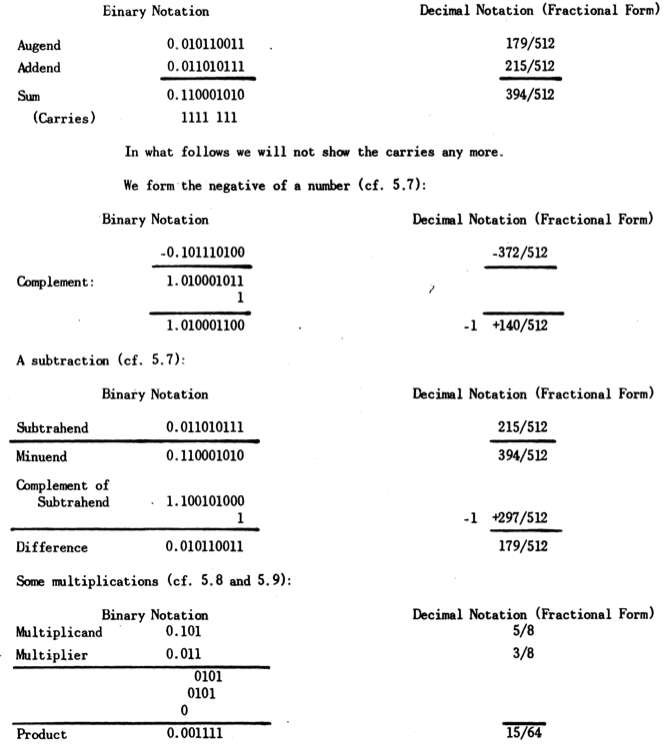
\includegraphics[width=160 mm]{Fig1-a}

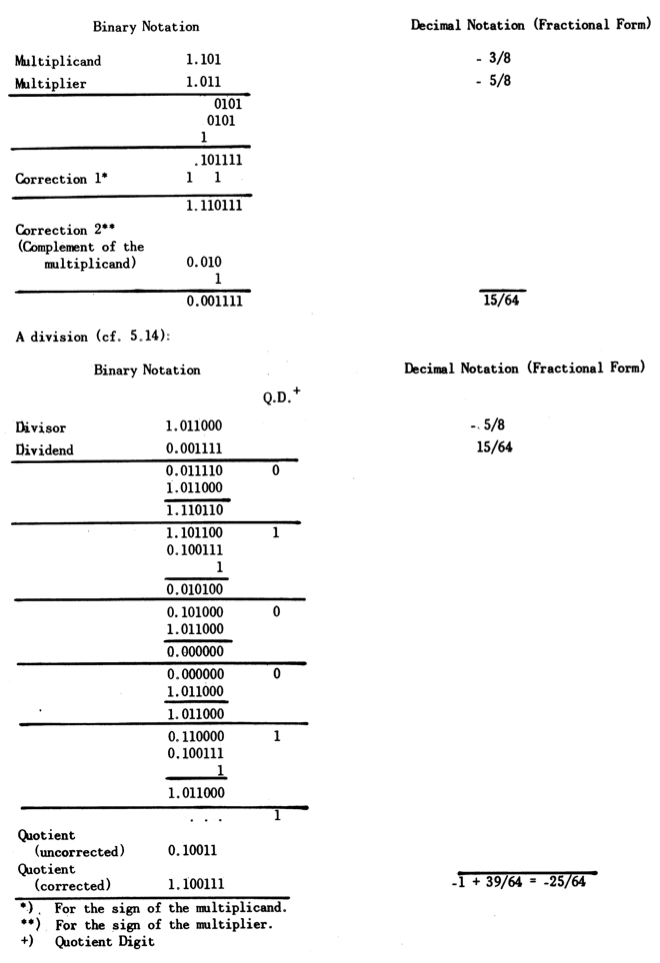
\includegraphics[width=160 mm]{Fig1-b}

Note that this deviates by $\frac{1}{64}$, i.e.\ by one unit of the right-most position, from the correct result $-\frac{3}{8}$. This is a consequence of our round-off rule, which forces the right-most digit to be 1 under all conditions. This occasionally produces results with unfamiliar and even annoying aspects (e.g.\ when quotients like $0:y$ or $y:y$ are formed), but it is nevertheless unobjectionable and self-consistent on the basis of our general principles.

\section{The Control}

\subsection{Introduction}
It has already been stated that the computer will contain an organ, called the Control, which can automatically execute the orders stored in the Selectrons. Actually, for a reason stated in 6.3, the orders for this computer are less than half as long as a forty binary digit number, and hence the orders are stored in the Selectron memory in pairs.

Let us consider the routine that the control performs in directing a computation. The control must know the location in the Selectron memory of the pair of orders to be executed. It must direct the Selectrons to transmit this pair of orders to the Selectron register and then to itself. It must then direct the execution of the operation specified in the first of the two orders. Among these orders we can immediately describe two major types: An order of the first type begins by causing the transfer of the number, which is stored at a specified memory location, from the Selectrons to the Selectron register. Next, it causes the arithmetical unit to perform some arithmetical operations on this number (usually in conjunction with another number which is already in the arithmetical unit), and to retain the resulting number in the arithmetical unit. The second type order causes the transfer of the number, which is held in the arithmetical unit, into the Selectron register, and from there to a specified memory location in the Selectrons. (It may also be that this latter operation will permit a direct transfer from the arithmetical unit into the Selectrons.) An additional type of order consists of the transfer orders of 3.5. Further orders control the inputs and the outputs of the machine. The process described at the beginning of this paragraph must then be repeated with the second order of the order pair. This entire routine is repeated until the end of the problem.

\subsection{Switching the memory}
It is clear from what has just been stated that the control must have a means of switching to a specified location in the Selectron memory, for withdrawing both numbers for the computation and pairs of orders. Since the Selectron memory (as tentatively planned) will hold $2^{12} = 4,096$ forty-digit words (a word is either a number or a pair of orders), a twelve-digit binary number suffices to identify a memory location. Hence a switching mechanism is required which will, on receiving a twelve-digit binary number, select the corresponding memory location.

The type of circuit we propose to use for this purpose is known as a decoding or many-one function table. It has been developed in various forms independently by J. Rajchman and P. Crawford. It consists of $n$ flip-flops which register an $n$-digit binary number. It also has a maximum of $2n$ output wires. The flip-flops activate a matrix in which the interconnections between input and output wires are made in such a way that one and only one of $2n$ output wires is selected (i.e.\ has a positive voltage applied to it). These interconnections may be established by means of resistors or by means of non-linear elements (such as diodes or rectifiers); all these various methods are under investigation. The Selectron is so designed that four such function table switches are required, each with a three digit entry and eight ($2^3$) outputs. Four sets of eight wires each are brought out of the Selectron for switching purposes, and a particular location is selected by making one wire positive with respect to the remainder. Since all forty Selectrons are switched in parallel, these four sets of wires may be connected directly to the four function table outputs.

\subsection{Decoding orders}
Since most computer operations involve at least one number located in the Selectron memory, it is reasonable to adopt a code in which twelve binary digits of every order are assigned to the specification of a Selectron location. In those orders which do not require a number to be taken out of or into the Selectrons these digit positions will not be used.

Though it has not been definitely decided how many operations will be built into the computer (i.e.\ how many different orders the control must be able to understand), it will be seen presently that there will probably be more than $2^5$ but certainly less than $2^6$. For this reason it is feasible to assign 6 binary digits for the order code. It thus turns out that each order must contain eighteen binary digits, the first twelve identifying a memory location and the remaining six specifying an operation. It can now be explained why orders are stored in the memory in pairs. Since the same memory organ is to be used in this computer for both orders and numbers, it is efficient to make the length of each about equivalent. But numbers of eighteen binary digits would not be sufficiently accurate for problems which this machine will solve. Rather, an accuracy of at least $10^{-10}$ or $2^{-33}$ is required. Hence it is preferable to make the numbers long enough to accommodate two orders.

As we pointed out in 2.3, and used in 4.2 \emph{et seq.} and 5.7 \emph{et seq.}, our numbers will actually have 40 binary digits each. This allows 20 binary digits for each order, i.e.\ the 12 digits that specify a memory location, and 8 more digits specifying the nature of the operation (instead of the minimum of 6 referred to above). It is convenient, as will be seen in 6.8.2. and Chapter 9, Part II to group these binary digits into \emph{tetrads}, groups of 4 binary digits. Hence a whole word consists of 10 tetrads, a half word or order of 5 tetrads, and of these 3 specify a memory location and the remaining 2 specify the nature of the operation. Outside the machine each tetrad can be expressed by a base 16 digit. (The base 16 digits are best designated by symbols of the 10 decimal digits 0 to 9, and 6 additional symbols, e.g.\ the letters a to f. Cf. Chapter 9, Part II.) These 16 characters should appear in the typing for and the printing from the machine. (For further details of these arrangements, \emph{cf. loc. cit.} above.)

The specification of the nature of the operation that is involved in an order occurs in binary form, so that another many-one or decoding function is required to decode the order. This function table will have six input flip-flops (the two remaining digits of the order are not needed). Since there will not be 64 different orders, not all 64 outputs need be provided. However, it is perhaps worthwhile to connect the outputs corresponding to unused order possibilities to a checking circuit which will give an indication whenever a code word unintelligible to the control is received in the input flip-flops.

The function table just described energizes a different output wire for each different code operation. As will be shown later, many of the steps involved in executing different orders overlap. (For example, addition, multiplication, division, and going from the Selectrons to the register all include transferring a number from the Selectrons to the Selectron register.) For this reason it is perhaps desirable to have an additional set of control wires, each of which is activated by any particular combination of different code digits. These may be obtained by taking the output wires of the many-one function table and using them to operate tubes which will in turn operate a one-many (or coding) function table. Such a function table consists of a matrix as before, but in this case only one of the input wires are activated. This particular table may be referred to as the recoding function table.

The twelve flip-flops operating the four function tables used in selecting a Selectron position, and the six flip-flops operating the function table used for decoding the order, are referred to as the \emph{Function Table Register}, FR.

\subsection{Transfer of orders to the Control}
Let us consider next the process of transferring a pair of orders from the Selectrons to the control. These orders first go into SR. The order which is to be used next may be transferred directly into FR. The second order of the pair must be removed from SR (since SR may be used when the first order is executed), but cannot as yet be placed in FR. Hence a temporary storage is provided for it. The storage means is called the \emph{Control Register}, CR, and consists of 20 (or possibly 18) flip-flops, capable of receiving a number from SR and transmitting a number to FR.

As already stated (6.1), the control must know the location of the pair of orders it is to get from the Selectron memory. Normally this location will be the one following the location of the two orders just executed. That is, until it receives an order to do otherwise, the control will take its orders from the Selectrons in sequence. Hence the order location may be remembered in a twelve stage binary counter (one capable of counting $2^12$) to which one unit is added whenever a pair of orders is executed. This counter is called the Control Counter, CC.

The details of the process of obtaining a pair of orders from the Selectron are thus as follows: The contents of CC are copied into FR, the proper Selectron location is selected, and the contents of the Selectrons are transferred to SR. FR is then cleared, and the contents of SR are transferred to it and CR. CC is advanced by one unit so the control will be prepared to select the next pair of orders from the memory. (There is, however, an exception from this last rule for the so-called transfer orders, cf. 3.5. This may feed CC in a different manner, cf. the next paragraph below.) First the order in FR is executed and then the order in CR is transferred to FR and executed. It should be noted that all these operations are directed by the control itself, not only the operations specified in the control words sent to FR, but also the automatic operations required to get the correct orders there.

Since the method by means of which the control takes order pairs in sequence from the memory has been described, it only remains to consider how the control shifts itself from one sequence of control orders to another in accordance with the operations described in 3.5. The execution of these operations is relatively simple. An order calling for one of these operations contains the twelve digit specification of the position to which the control is to be switched, and these digits will appear in the left-hand twelve flip-flops of FR. All that is required to shift the control is to transfer the contents of these flip-flops to CC. When the control goes to the Selectrons for the next pair of orders it will then go to the location specified by the number so transferred. In the case of the unconditional transfer, the transfer is made automatically; in the case of the conditional transfer it is made only if the sign counter of the Accumulator registers zero.

\subsection{Synchronized Control circuits}
In this report we will discuss only the general method by means of which the control will execute specific orders, leaving the details until later. It has already been explained (5.5) that when a circuit is to be designed to accomplish a particular elementary operation (such as addition), a choice must be made between a static type and a dynamic type circuit. When the design of the control is considered, this same choice arises. The function of the control is to direct a sequence of operations which take place in the various circuits of the computer (including the circuits of the control itself). Consider what is involved in directing an operation. The control must signal for the operation to begin, it must supply whatever signals are required to specify that particular operation, and it must in some way know when the operation has been completed so that it may start the succeeding operation. Hence the control circuits must be capable of timing the operations. It should be noted that timing is required whether the circuit performing the operation is static or dynamic. In the case of a static type circuit the control must supply static control signals for a period of time sufficient to allow the output voltages to reach the steady-state condition. In the case of a dynamic type circuit the control must send various pulses at proper intervals to this circuit.

If all circuits of a computer are static in character, the control timing circuits may likewise be static, and no pulses are needed in the system. However, though some of the circuits of the computer we are planning will be static, they will probably not all be so, and hence pulses as well as static signals must be supplied by the control to the rest of the computer. There are many advantages in deriving these pulses from a central source, called the clock. The timing may then be done either by means of counters counting clock pulses or by means of electrical delay lines (an RC circuit is here regarded as a simple delay line). Since the timing of the entire computer is governed by a single pulse source, the computer circuits will be said to operate as a synchronized system.

The clock plays an important role both in detecting and in localizing the errors made by the computer. One method of checking which is under consideration is that of having two identical computers which operate in parallel and automatically compare each other's results. Both machines would be controlled by the same clock, so they would operate in absolute synchronism. It is not necessary to compare every flip-flop of one machine with the corresponding flip-flop of the other. Since all numbers and control words pass through either the Selectron register or the accumulator soon before or soon after they are used, it suffices to check the flip-flops of the Selectron register and the flip-flops of the accumulator which hold the number registered there; in fact, it seems possible to check the accumulator only (cf. the end of 6.6.2). The checking circuit would stop the clock whenever a difference appeared, or stop the machine in a more direct manner if an asynchronous system is used. Every flip-flop of each computer will be located at a convenient place. In fact, all neons will be located on one panel, the corresponding neons of the two machines being placed in parallel rows so that one can tell at a glance (after the machine has been stopped) where the discrepancies are.

The merits of any checking system must be weighed against its cost. Building two machines may appear to be expensive, but since most of the cost of a scientific computer lies in development rather than production, this consideration is not so important as it might seem. Experience may show that for most problems the two machines need not be operated in parallel. Indeed, in most cases purely mathematical, external checks are possible: Smoothness of the results, behavior of differences of various types, validity of suitable identities, redundant calculations, etc. All of these methods are usually adequate to disclose the presence or absence of error \emph{in toto}; their drawback is only that they may not allow the detailed diagnosing and locating of errors at all or with ease. When a problem is run for the first time, so that it requires special care, or when an error is known to be present, and has to be located-only then will it be necessary as a rule, to use both machines in parallel. Thus they can be used as separate machines most of the time. The essential feature of such a method of checking lies in the fact that it checks the computation at every point (and hence detects transient errors as well as steady-state ones) and stops the machine when the error occurs so that the process of localizing the fault is greatly simplified. These advantages are only partially gained by duplicating the arithmetic part of the computer, or by following one operation with the complement operation (multiplication by division, etc.), since this fails to check either the memory or the control (which is the most complicated, though not the largest, part of the machine).

The method of localizing errors, either with or without a duplicate machine, needs further discussion. It is planned to design all the circuits (including those of the control) of the computer so that if the clock is stopped between pulses the computer will retain all its information in flip-flops so that the computation may proceed unaltered when the clock is started again. This principle has already demonstrated its usefulness in the ENIAC. This makes it possible for the machine to compute with the clock operating at any speed below a certain maximum, as long as the clock gives out pulses of constant shape regardless of the spacing between pulses. In particular, the spacing between pulses may be made indefinitely large. The clock will be provided with a mode of operation in which it will emit a single pulse whenever instructed to do so by the operator. By means of this, the operator can cause the machine to go through an operation step by step, checking the results by means of the indicating-lamps connected to the flip-flops. It will be noted that this design principle does not exclude the use of delay lines to obtain delays as long as these are only used to time the constituent operations of a single step, and have no part in determining the machine's operating repetition rate. Timing coincidences by means of delay lines is excluded since this requires a constant pulse rate.

\subsection{Orders for the internal operations}
The orders which the control understands may be divided into two groups: Those that specify operations which are performed within the computer and those that specify operations involved in getting data into and out of the computer. At the present time the internal operations are more completely planned than the input and output operations, and hence they will be discussed more in detail than the latter (which are treated briefly in 6.8). The internal operations which have been tentatively adopted are listed in Table 1. It has already been pointed out that not all of these operations are logically basic, but that many can be programmed by means of others. In the case of some of these operations the reasons for building them into the control have already been given. In this section we will give reasons for building the other operations into the control and will explain in the case of each operation what the control must do in order to execute it.

In order to have the precise mathematical meaning of the symbols which are introduced in what follows clearly in mind, the reader should consult the table at the end of the report for each new symbol, in addition to the explanations given in the text.

\subsubsection{Addition}
Throughout what follows $S(x)$ will denote the memory location No. $x$ in the Selectron. Accordingly the $x$ which appears in $S(x)$ is a 12-digit binary, in the sense of 6.2. The eight addition operations $[S(x) \rightarrow Ac +,\ S(x) \rightarrow Ac-,\ S(x) \rightarrow Ah+,\ S(x) \rightarrow Ah-,\ S(x) \rightarrow Ac + M,\ S(x) \rightarrow Ac- M,\ S(x) \rightarrow Ah + M,\ S(x) \rightarrow Ah - M]$ involves the following possible four steps:

\emph{First:} Clear SR and transfer into it the number at $S(x)$.

\emph{Second:} Clear Ac if the order contains the symbol $C$; do not clear Ac if the order contains the symbol $h$.

\emph{Third:} Add the number in SR or its negative (i.e.\ in our present system its complement with respect to $2^1$) into Ac. If the order does not contain the symbol $M$, use the number in SR or its negative according to whether the order contains the symbol + or $-$. If the order contains the symbol $M$, use the number in SR or its negative according to whether the sign of the number in SR and the symbol + or $-$ in the order do or do not agree.

\emph{Fourth:} Perform a complete carry. Building the last four addition operations (those containing the symbol $M$) into the control is fairly simple: It calls only for one extra comparison (of the sign in SR and the + or $-$ in the order, cf. the third step above), and it requires, therefore, only a few tubes more than required for the first four addition operations (those not containing the symbol $M$). These facts would seem of themselves to justify adding the operations in question: plus and minus the absolute value. But it should be noted that these operations can be programmed out of the other operations of Table 1 with correspondingly few orders (three for absolute value and five for minus absolute value), so that some further justification for building them in is required. The absolute value order is frequently in connection with the orders L and R (see 6.6.7), while the minus absolute value order makes the detection of a zero very simple by merely detecting the sign of $-|N|$. (If $-|N| \geqq 0$, then $N = 0$.)

\subsubsection{Register transfers}
The operation of $S(x) \rightarrow R$ involves the following two steps:

\emph{First:} Clear SR, and transfer $S(x)$ to it.

\emph{Second:} Clear AR and add the number in the Selectron register into it. The operation of $R \rightarrow Ac$ merits more detailed discussion, since there are alternative ways of removing numbers from AR. Such numbers could be taken directly to the Selectrons as well as into Ac, and they could be transferred to Ac in parallel, in sequence, or in sequence parallel. It should be recalled that while most of the numbers that go into AR have come from the Selectrons and thus need not be returned to them, the result of a division and the right-hand 39 digits of a product appear in AR. Hence while an operation for withdrawing a number from AR is required, it is relatively infrequent and therefore need not be particularly fast. We are therefore considering the possibility of transferring at least partially in sequence and of using the shifting properties of Ac and of AR for this. Transferring the number to the Selectron via the accumulator is also desirable if the dual machine method of checking is employed, for it means that even if numbers are only checked in their transit through the accumulator, nevertheless every number going into the Selectron is checked before being placed there.

\subsubsection{Multiplication}
The operation $S(x) \times R \rightarrow Ac$ involves the following six steps:

\emph{First:} Clear SR and transfer $S(x)$ (the multiplicand) into it.

\emph{Second:} Thirty-nine steps, each of which consist of the two following parts: (a) Add (or rather shift) the sign digit of SR into the partial product in Ac, or add all but the sign digit of SR into the partial product in Ac---depending upon whether the right-most digit in AR is 0 or 1---and effect the appropriate carries. (b) Shift Ac and AR to the right, fill the sign digit of Ac with a 0 and the digit of AR immediately right of the sign digit (positional value $2^{-1}$) with the previously right-most digit of Ac. (There are ways to save time by merging these two operations when the right-most digit in Ar is 0, but we will not discuss them here more fully.)

\emph{Third:} If the sign digit in SR is 1 (i.e.\ $-$), then inject a carry into the right-most stage of Ac and place a 1 into the sign digit of Ac.

\emph{Fourth:} If the original sign digit of AR is 1 (i.e.\ $-$), then subtract the contents of SR from Ac.

\emph{Fifth:} If a partial carry system was employed in the main process, then a complete carry is necessary at the end.

\emph{Sixth:} The appropriate round-off must be effected. (Cf. Chapter 9, Part II, for details, where it is also explained how the sign digit of the Arithmetic register is treated as part of the round-off process.)

It will be noted that since any number held in Ac at the beginning of the process is gradually shifted into AR, it is impossible to accumulate sums of products in Ac without storing the various products temporarily in the Selectrons. While this is undoubtedly a disadvantage, it cannot be eliminated without constructing an extra register, and this does not at this moment seem worthwhile.

On the other hand, saving the right-hand 39 digits of the answer is accomplished with very little extra equipment, since it means connecting the $2^{-39}$ stage of Ac to the $2^{-1}$ stage of AR during the shift operation. The advantage of saving these digits is that it simplifies the handling of numbers of any number of digits in the computer (cf. the last part of 5.12). Any number of $39k$ binary digits (where $k$ is an integer) and sign can be divided into $k$ parts, each part being placed in a separate Selectron position. Addition and subtraction of such numbers may be programmed out of a series of additions or subtractions of the 39-digit parts, the carry-over being programmed by means of $Cc \rightarrow S(x)$ and $Cc' \rightarrow S(x)$ operations. (If the $2^0$ stage of Ac registers negative after the addition of two 39-digit parts, a carry-over has taken place and hence $2^{-39}$ must be added to the sum of the next parts.) A similar procedure may be followed in multiplication if all 78 digits of the product of the two 39-digit parts are kept, as is planned. (For the details, cf. Chapter 9, Part II.) Since it would greatly complicate the computer to make provision for holding and using a 78 digit dividend, it is planned to program $39k$ digit division in one of the ways described at the end of 5.12.

\subsubsection{Division}
The operation of division $Ac \div S(x) \rightarrow R$ involves the following four steps:

\emph{First:} Clear SR and transfer $S(x)$ (the divisor) into it.

\emph{Second:} Clear AR.

\emph{Third:} Thirty-nine steps, each of which consists of the following three parts: (a) Sense the signs of the contents of Ac (the partial remainder) and of SR, and sense whether they agree or not. (b) Shift Ac and AR left. In this process the previous sign digit of Ac is lost. Fill the right-most digit of Ac (after the shift) with a 0, and the right-most digit of AR (before the shift) with 0 or 1, depending on whether there was disagreement or agreement in (a). (c) Add or subtract the contents of SR into Ac, depending on the same alternative as above.

\emph{Fourth:} Fill the right-most digit of AR with a 1, and change its sign digit.

For the purpose of timing the 39 steps involved in division a six-stage counter (capable of counting to $2^6 = 64$) will be built into the control. This same counter will also be used for timing the 39 steps of multiplication, and possibly for controlling Ac when a number is being transferred between it and a tape in either direction (see 6.8.).

\subsubsection{Memory substitution}
The three substitution operations [$At \rightarrow S(x)$, $Ap \rightarrow S(x)$, and $Ap' \rightarrow S(x)$] involve transferring all or part of the number held in Ac into the Selectrons. This will be done by means of gate tubes connected to the registering flip-flops of Ac. Forty such tubes are needed for the total substitutions, $At \rightarrow S(x)$. The partial substitution $Ap \rightarrow S(x)$ and $Ap' \rightarrow S(x)$ requires that the left-hand twelve digits of the number held in Ac be substituted in the proper places in the left-hand and right-hand orders, respectively. This may be done by means of extra gate tubes, or by shifting the number in Ac and using the gate tubes required for $At \rightarrow S(x)$. (This scheme needs some additional elaboration, when the order directing and the order suffering the substitution are the two successive halves of the same word; i.e.\ when the latter is already in FR at the time when the former becomes operative in CR, so that the substitution effected in the Selectrons comes too late to alter the order which has already reached CR, to become operative at the next step in FR. There are various ways to take care of this complication, either by some additional equipment or by appropriate prescriptions in coding. We will not discuss them here in more detail, since the decisions in this respect are still open.)

The importance of the partial substitution operations can hardly be overestimated. It has already been pointed out (3.3) that they allow the computer to perform operations it could not otherwise conveniently perform, such as making use of a function table stored in the Selectron memory. Furthermore, these operations remove a very sizable burden from the person coding problems, for they make possible the coding of classes of problems in contrast to coding each individual problem separately. Because $Ap \rightarrow S(x)$ and $Ap' \rightarrow S(x)$ are available, any program sequence may be stated in general form (that is, without Selectron location designations for the numbers being operated on) and the Selectron locations of the numbers to be operated on substituted whenever that sequence is used. As an example, consider a general code for $n$-th order integration of $m$ total differential equations for $p$ steps of independent variable $t$, formulated in advance. Whenever a problem requiring this rule is coded for the computer, the general integration sequence can be inserted into the statement of the problem along with coded instructions for telling the sequence where it will be located in the memory [so that the proper $S(x)$ designations will be inserted into such orders as $Cu \rightarrow S(x)$, etc.]. Whenever this sequence is to be used by the computer it will automatically substitute the correct values of $m$, $n$, $p$ and $\Delta t$, as well as the locations of the boundary conditions and the descriptions of the differential equations, into the general sequence. (For the details of this particular procedure, cf. Chapter 13, Part II.) A library of such general sequences will be built up, and facilities provided for convenient insertion of any of these into the coded statement of a problem (cf. 6.8.4). When such a scheme is used, only the distinctive features of a problem need be coded.

\subsubsection{Shift of Control}
The manner in which the control shift operations [$Cu \rightarrow S(x)$, $Cu' \rightarrow S(x)$, $Cc \rightarrow S(x)$, and $Cc' \rightarrow S(x)$] are realized has been discussed in 6.4 and needs no further comment.

\subsubsection{Unit shifts and the floating binary point}
One basic question which must be decided before a computer is built is whether the machine is to have a so-called floating binary (or decimal) point. While a floating binary point is undoubtedly very convenient in coding problems, building it into the computer adds greatly to its complexity and hence a choice in this matter should receive very careful attention. However, it should first be noted that the alternatives ordinarily considered (building a machine with a floating binary point vs. doing all computation with a fixed binary point) are not exhaustive and hence that the arguments generally advanced for the floating binary point are only of limited validity. Such arguments overlook the fact that the choice with respect to any particular operation (except for certain basic ones) is not between building it into the computer and not using it at all, but rather between building it into the computer and programming it out of operations built into the computer. (One short reference to the floating binary point was made in 5.13.)

Building a floating binary point into the computer will not only complicate the control but will also increase the length of a number and hence increase the size of the memory and the arithmetic unit. Every number is effectively increased in size, even though the floating binary point is not needed in many instances. Furthermore, there is considerable redundancy in a floating binary point type of notation, for each number carries with it a scale factor, while generally speaking a single scale factor will suffice for a possibly extensive set of numbers. By means of the operations already described in the report a floating binary point can be programmed. While additional memory capacity is needed for this, it is probably less than that required by a built-in floating binary point since a different scale factor does not need to be remembered for each number.

To program a floating binary point involves detecting where the first zero occurs in a number in Ac. Since Ac has shifting facilities this can best be done by means of them. In terms of the operations previously described this would require taking the given number out of Ac and performing a suitable arithmetical operation on it: For a (multiple) right shift a multiplication, for a (multiple) left shift either one division, or as many doublings (i.e. additions) as the shift has stages. However, these operations are inconvenient and time-consuming, so we propose to introduce two operations (L and R) in order that this (i.e. the single left and right shift) can be accomplished directly. These operations make use of facilities already present in Ac and hence add very little equipment to the computer. It should be noted that in many instances a single use of L and possibly of R will suffice in programming a floating binary point. For if the two factors in a multiplication have no superfluous zeros, the product will have at most one superfluous zero (if $\frac{1}{2} \leqq X < 1$ and $\frac{1}{2} \leqq Y < 1$, then $\frac{1}{4} \leqq XY < 1$). This is similarly true in division (if $\frac{1}{4} \leqq X < \frac{1}{2}$ and $\frac{1}{2} \leqq Y < 1$, then $\frac{1}{4} < X/Y < 1$). In addition and subtraction any numbers growing out of range can be treated similarly. Numbers which decrease in these cases, i.e.\ develop a sequence of zeros at the beginning, are really (mathematically) losing precision. Hence it is perfectly proper to omit formal readjustments in this event. (Indeed, such a true loss of precision cannot be obviated by any formal procedure, but, if at all, only by a different mathematical formulation of the problem.)

\subsection{Timing circuits}
Table 1 shows that many of the operations which the control is to execute have common elements. Thus addition, subtraction, multiplication and division all involve transferring a number from the Selectrons to SR. Hence the control may be simplified by breaking some of the operations up into more basic ones. A timing circuit will be provided for each basic operation, and one or more such circuits will be involved in the execution of an order. The exact choice of basic operations will depend upon how the arithmetic unit is built.

In addition to the timing circuits needed for executing the orders of Table 1, two such circuits are needed for the automatic operations of transferring orders from the Selectron register to CR and FR, and for transferring an order from CR to FR. In normal computer operation these two circuits are used alternately, so a binary counter is needed to remember which is to be used next. In the operations $Cu' \rightarrow S(x)$ and $Cc \rightarrow S(x)$ the first order of a pair is ignored, so the binary counter must be altered accordingly.

The execution of a sequence of orders involves using the various timing circuits in sequence. When a given timing circuit has completed its operation, it emits a pulse which should go to the timing circuit to be used next. Since this depends upon the particular operation being executed, these pulses are routed according to the signals received from the decoding and recoding function tables activated by the six binary digits specifying an order.

\subsection{Input-output orders}
In this section we will consider what must be added to the control so that it can direct the mechanisms for getting data into and out of the computer and also describe the mechanisms themselves. Three different kinds of input-output mechanisms are planned.

\emph{First:} Several magnetic wire storage units operated by servo-mechanisms controlled by the computer.

\emph{Second:} Some viewing tubes for graphical portrayal of results.

\emph{Third:} A typewriter for feeding data directly into the computer, not to be confused with the equipment used for preparing and printing from magnetic wires. As presently planned the latter will consist of modified Teletypewriter equipment, cf. 6.8.2 and 6.8.4.

\subsubsection{Wire orders}
Since there already exists a way of transferring numbers between the Selectrons and Ac, therefore Ac may be used for transferring numbers from and to a wire. The latter transfer will be done serially and will make use of the shifting facilities of Ac. Using Ac for this purpose eliminates the possibility of computing and reading from or writing on the wires simultaneously. However, simultaneous operation of the computer and the input-output organ requires additional temporary storage and introduces a synchronizing problem, and hence it is not being considered for the first model.

Since, at the beginning of the problem, the computer is empty, facilities must be built into the control for reading a set of numbers from a wire when the operator presses a manual switch. As each number is read from a wire into Ac, the control must transfer it to its proper location in the Selectrons. The CC may be used to count off these positions in sequence, since it is capable of transmitting its contents to FR. A detection circuit on CC will stop the process when the specified number of numbers has been placed n the memory, and the control will then be shifted to the orders located in the first position of the Selectron memory.

It has already been stated that the entire memory facilities of the wires should be available to the computer without human intervention. This means that the control must be able to select the proper set of numbers from those going by. Hence additional orders are required for the code. Here, as before, we are faced with two alternatives. We can make the control capable of executing an order of the form: Take numbers from positions $p$ to $p + s$ on wire No.\ $k$ and place them in Selectron locations $v$ to $v + s$. Or we can make the control capable of executing some less complicated operations which, together with the already given control orders, are sufficient for programming the transfer operation of the first alternative. Since the latter scheme is simpler we adopt it tentatively.

The computer must have some way of finding a particular number on a wire. One method of arranging for this is to have each number carry with it its own location designation. A method more economical of wire memory capacity is to use the Selectron memory facilities to remember the position of each wire. For example, the computer would hold the number $t_1$ specifying which number on the wire is in position to be read. If the control is instructed to read the number at position $p_1$ on this wire, it will compare $p_1$ with $t_1$ and if they differ, cause the wire to move in the proper direction. As each number on the wire passes by, one unit is added or subtracted to $t_1$ and the comparison repeated. When $p_1 = t_1$ numbers will be transferred from the wire to the accumulator and then to the proper location in the memory. Then both $t_1$ and $p_1$ will be increased by 1, and the transfer from the wire to accumulator to memory repeated. This will be iterated, until $t_1 + s$ and $p_1 + s$ are reached, at which time the control will direct the wire to stop.

Under this system the control must be able to execute the following orders with regard to each wire: Start the wire forward, start the wire in reverse, stop the wire, transfer from wire to Ac, and transfer from Ac to wire. In addition, the wire must signal the control as each digit is read and when the end of a number has been reached. Conversely, when recording is done the control must have a means of timing the signals sent from Ac to the wire, and of counting off the digits. The $2^6$ counter used for multiplication and division may be used for the latter purpose, but other timing circuits will be required for the former.

If the method of checking by means of two computers operating simultaneously is adopted, and each machine is built so that it can operate independently of the other, then each will have a separate input-output mechanism. The process of making wires for the computer must then be duplicated, and in this way the work of the person making a wire can be checked. Since the wire servomechanisms cannot be synchronized by the central clock, a problem of synchronizing the two computers when the wires are being used arises. It is probably not practical to synchronize the wire feeds to within a given digit, but this is unnecessary since the numbers coming into the two organs Ac need not be checked as the individual digits arrive, but only prior to being deposited in the Selectron memory.

\subsubsection{Binary decimal conversion}
Since the computer operates in the binary system, some means of decimal-binary and binary-decimal conversions is highly desirable. Various alternative ways of handling this problem have been considered. In general we recognize two broad classes of solutions to this problem.

\emph{First:} The conversion problems can be regarded as simple arithmetic processes and programmed as sub-routines out of the orders already incorporated in the machine. The details of these programs together with a more complete discussion are given fully in Chapter 9, Part II, where it is shown, among other things, that the conversion of a word takes about 5 m sec. Thus the conversion time is comparable to the reading or withdrawing time for a word---about 2 m sec---and is trivial as compared to the solution time for problems to be handled by the computer. It should be noted that the treatment proposed there presupposes only that the decimal data presented to or received from the computer are in tetrads, each tetrad being the binary coding of a decimal digit---the information (precision) represented by a decimal digit being actually equivalent to that represented by 3.3 binary digits. The coding of decimal digits into tetrads of binary digits and the printing of decimal digits from such tetrads can be accomplished quite simply and automatically by slightly modified Teletype equipment, cf. 6.8.4 below.

\emph{Second:} The conversion problems can be regarded as unique problems and handled by separate conversion equipment incorporated either in the computer proper or associated with the mechanisms for preparing and printing from magnetic wires. Such converters are really nothing other than special purpose digital computers. They would seem to be justified only for those computers which are primarily intended for solving problems in which the computation time is small compared to the input-output time, to which class our computer does not belong.

\subsubsection{Viewing tubes}
It is possible to use various types of cathode ray tubes, and in particular Selectrons for the viewing tubes, in which case programming the viewing operation is quite simple. The viewing Selectrons can be switched by the same function tables that switch the memory Selectrons. By means of the substitution operation $Ap \rightarrow S(x)$ and $Ap' \rightarrow S(x)$, six-digit numbers specifying the abscissa and ordinate of the point (six binary digits represent a precision of one part in $2^6 = 64$, i.e.\ of about $1.5\%$ which seems reasonable in such a component) can be substituted in this order, which will specify that a particular one of the viewing Selectrons is to be activated.

\subsubsection{Input-output equipment}
As was mentioned above, the mechanisms used for preparing and printing from wire for the first model, at least, will be modified Teletype equipment. We are quite fortunate in having secured the full cooperation of the Ordnance Development Division of the National Bureau of Standards in making these modifications and in designing and building some associated equipment.

By means of this modified Teletype equipment an operator first prepares a checked paper tape and then directs the equipment to transfer the information from the paper tape to the magnetic wire. Similarly a magnetic wire can transfer its contents to a paper tape which can be used to operate a teletypewriter. (Studies are being undertaken to design equipment that will eliminate the necessity for using paper tapes.)

As was shown in 6.6.5, the statement of a new problem on a wire involves data unique to that problem interspersed with data found on previously prepared paper tapes or magnetic wires. The equipment discussed in the previous paragraph makes it possible for the operator to combine conveniently these data on to a single magnetic wire ready for insertion into the computer.

It is frequently very convenient to introduce data into a computation without producing a new wire. Hence it is planned to build one simple typewriter as an integral part of the computer. By means of this typewriter the operator can stop the computation, type in a memory location (which will go to the FR), type in a number (which will go to Ac and then be placed in the first mentioned location), and start the computation again.

\subsubsection{Finish signal}
There is one further order that the control needs to execute. There should be some means by which the computer can signal to the operator when a computation has been concluded, or when the computation has reached a previously determined point. Hence an order is needed which will tell the computer to stop and to flash a light or ring a bell.
\raggedbottom

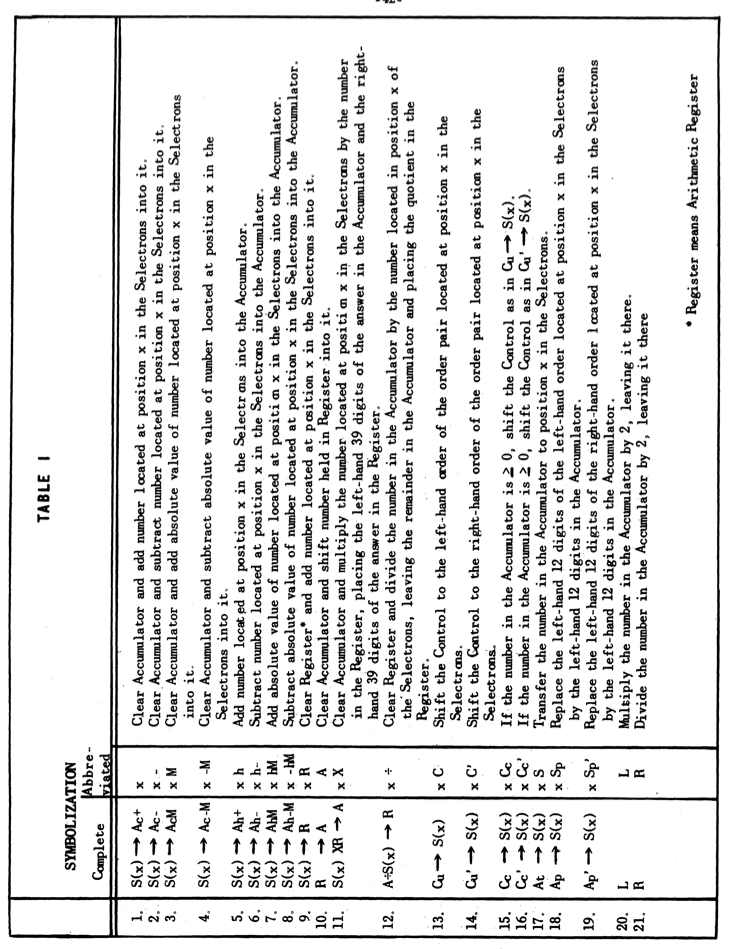
\includegraphics[width=160 mm]{Table-1}

\end{document}
